\documentclass[journal=jpcbfk,manuscript=article]{achemso}

%%%%%%%%%%%%%%%%%%%%%%%%%%%%%%%%%%%%%%%%%%%%%%%%%%%%%%%%%%%%%%%%%%%%%
%% Place any additional packages needed here.  Only include packages
%% which are essential, to avoid problems later. Do NOT use any
%% packages which require e-TeX (for example etoolbox): the e-TeX
%% extensions are not currently available on the ACS conversion
%% servers.
%%%%%%%%%%%%%%%%%%%%%%%%%%%%%%%%%%%%%%%%%%%%%%%%%%%%%%%%%%%%%%%%%%%%%
\usepackage[version=3]{mhchem} % Formula subscripts using \ce{}
\usepackage[T1]{fontenc}       % Use modern font encodings

%%%%%%%%%%%%%%%%%%%%%%%%%%%%%%%%%%%%%%%%%%%%%%%%%%%%%%%%%%%%%%%%%%%%%
%% If issues arise when submitting your manuscript, you may want to
%% un-comment the next line.  This provides information on the
%% version of every file you have used.
%%%%%%%%%%%%%%%%%%%%%%%%%%%%%%%%%%%%%%%%%%%%%%%%%%%%%%%%%%%%%%%%%%%%%
%%\listfiles

%%%%%%%%%%%%%%%%%%%%%%%%%%%%%%%%%%%%%%%%%%%%%%%%%%%%%%%%%%%%%%%%%%%%%
%% Place any additional macros here.  Please use \newcommand* where
%% possible, and avoid layout-changing macros (which are not used
%% when typesetting).
%%%%%%%%%%%%%%%%%%%%%%%%%%%%%%%%%%%%%%%%%%%%%%%%%%%%%%%%%%%%%%%%%%%%%
% \newcommand*\mycommand[1]{\texttt{\emph{#1}}}

%%%%%%%%%%%%%%%%%%%%%%%%%%%%%%%%%%%%%%%%%%%%%%%%%%%%%%%%%%%%%%%%%%%%%
%% Meta-data block
%% ---------------
%% Each author should be given as a separate \author command.
%%
%% Corresponding authors should have an e-mail given after the author
%% name as an \email command. Phone and fax numbers can be given
%% using \phone and \fax, respectively; this information is optional.
%%
%% The affiliation of authors is given after the authors; each
%% \affiliation command applies to all preceding authors not already
%% assigned an affiliation.
%%
%% The affiliation takes an option argument for the short name.  This
%% will typically be something like "University of Somewhere".
%%
%% The \altaffiliation macro should be used for new address, etc.
%% On the other hand, \alsoaffiliation is used on a per author basis
%% when authors are associated with multiple institutions.
%%%%%%%%%%%%%%%%%%%%%%%%%%%%%%%%%%%%%%%%%%%%%%%%%%%%%%%%%%%%%%%%%%%%%
\author{Kyle A. Barlow}
\affiliation{Graduate Program in Bioinformatics, University of California San Francisco, San Francisco, California, United States of America}
\email{kb@kylebarlow.com}
\author{Other Authors To Be Added}
\affiliation{Graduate Program in Bioinformatics, University of California San Francisco, San Francisco, California, United States of America}
\author{Tanja Kortemme}
\affiliation[QB3]{California Institute for Quantitative Biosciences, University of California San Francisco, San Francisco, California, United States of America}
\alsoaffiliation{Department of Bioengineering and Therapeutic Sciences, University of California San Francisco, San Francisco, California, United States of America}
\alsoaffiliation{Graduate Program in Bioinformatics, University of California San Francisco, San Francisco, California, United States of America}
\alsoaffiliation{Graduate Program in Biophysics, University of California San Francisco, San Francisco, California, United States of America}
\email{kortemme@cgl.ucsf.edu}

%%%%%%%%%%%%%%%%%%%%%%%%%%%%%%%%%%%%%%%%%%%%%%%%%%%%%%%%%%%%%%%%%%%%%
%% The document title should be given as usual. Some journals require
%% a running title from the author: this should be supplied as an
%% optional argument to \title.
%%%%%%%%%%%%%%%%%%%%%%%%%%%%%%%%%%%%%%%%%%%%%%%%%%%%%%%%%%%%%%%%%%%%%
\title[]
  {Flex ddG: Rosetta ensemble-based estimation of changes in protein-protein binding affinity upon mutation}

%%%%%%%%%%%%%%%%%%%%%%%%%%%%%%%%%%%%%%%%%%%%%%%%%%%%%%%%%%%%%%%%%%%%%
%% Some journals require a list of abbreviations or keywords to be
%% supplied. These should be set up here, and will be printed after
%% the title and author information, if needed.
%%%%%%%%%%%%%%%%%%%%%%%%%%%%%%%%%%%%%%%%%%%%%%%%%%%%%%%%%%%%%%%%%%%%%
% \abbreviations{}
% \keywords{}

%%%%%%%%%%%%%%%%%%%%%%%%%%%%%%%%%%%%%%%%%%%%%%%%%%%%%%%%%%%%%%%%%%%%%
%% The manuscript does not need to include \maketitle, which is
%% executed automatically.
%%%%%%%%%%%%%%%%%%%%%%%%%%%%%%%%%%%%%%%%%%%%%%%%%%%%%%%%%%%%%%%%%%%%%
\begin{document}

%%%%%%%%%%%%%%%%%%%%%%%%%%%%%%%%%%%%%%%%%%%%%%%%%%%%%%%%%%%%%%%%%%%%%
%% The "tocentry" environment can be used to create an entry for the
%% graphical table of contents. It is given here as some journals
%% require that it is printed as part of the abstract page. It will
%% be automatically moved as appropriate.
%%%%%%%%%%%%%%%%%%%%%%%%%%%%%%%%%%%%%%%%%%%%%%%%%%%%%%%%%%%%%%%%%%%%%
\begin{tocentry}
    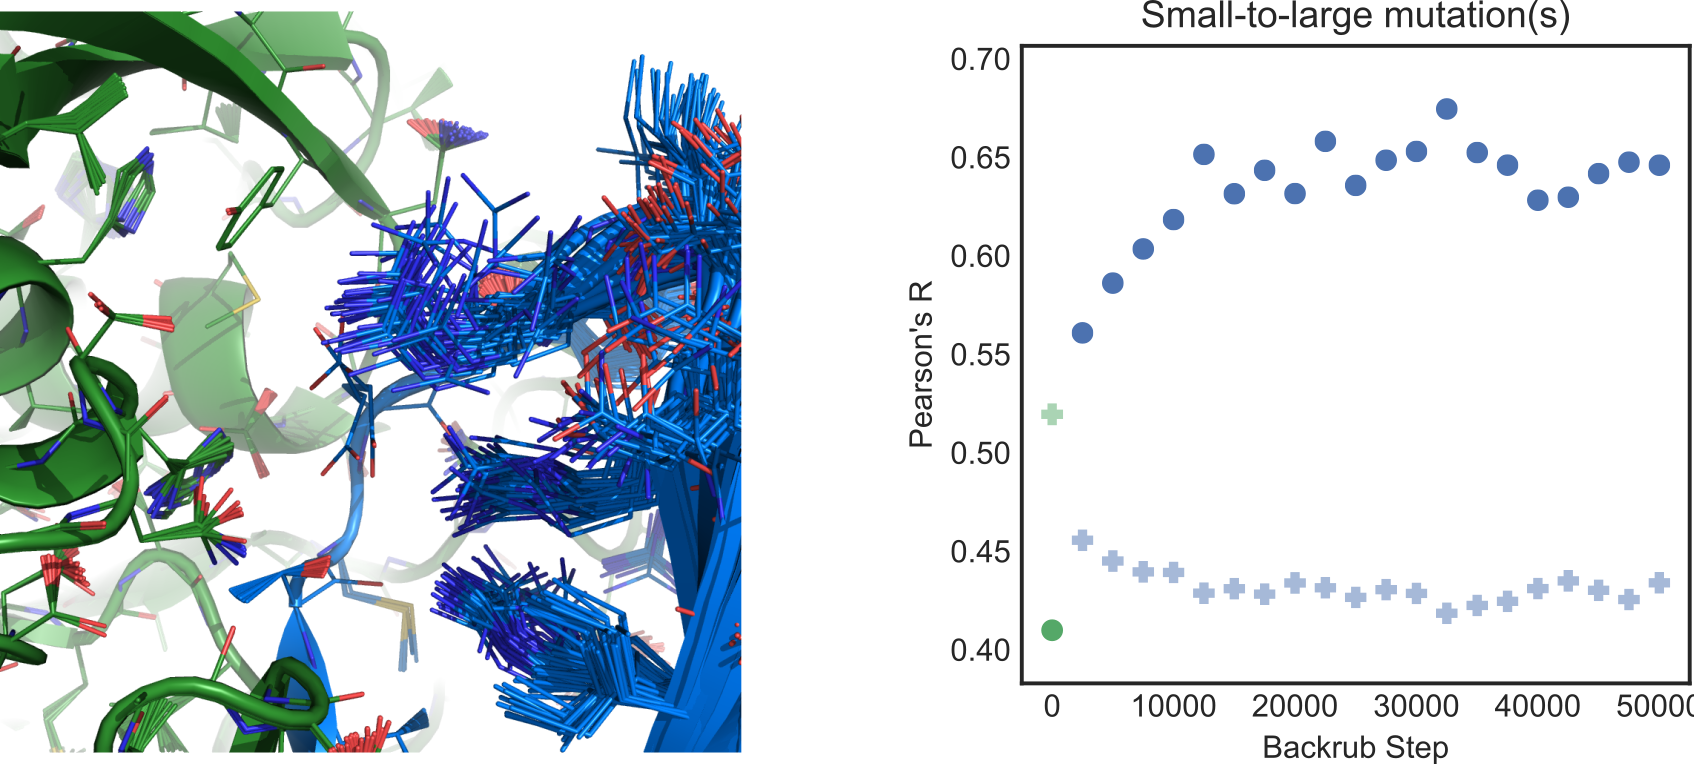
\includegraphics[width=0.8\textwidth,keepaspectratio]{figures/toc.png}
\end{tocentry}

%%%%%%%%%%%%%%%%%%%%%%%%%%%%%%%%%%%%%%%%%%%%%%%%%%%%%%%%%%%%%%%%%%%%%
%% The abstract environment will automatically gobble the contents
%% if an abstract is not used by the target journal.
%%%%%%%%%%%%%%%%%%%%%%%%%%%%%%%%%%%%%%%%%%%%%%%%%%%%%%%%%%%%%%%%%%%%%
\begin{abstract}
  Computational predicting changes in binding free energy of protein-protein interfaces after mutation allows these interactions to be designed and predicted in high throughput.
We have developed a method to predict these interface $\Delta\Delta G$s
Considering natural conformational plasticity could be helpful.
We developed a method to do this in Rosetta, using backrub based conformational sampling.
On a benchmark set of 1240 mutants, we measured performance, and were able to do better leading Rosetta methods.
On the subset of small to large, even better.
Considering flexibility was important, as a control method had a worse performance.
Averaging across more structures also improved performance.
Maching learning score function fitting also might show how the Rosetta energy function can be improved in the future.

\end{abstract}

%%%%%%%%%%%%%%%%%%%%%%%%%%%%%%%%%%%%%%%%%%%%%%%%%%%%%%%%%%%%%%%%%%%%%
%% Start the main part of the manuscript here.
%%%%%%%%%%%%%%%%%%%%%%%%%%%%%%%%%%%%%%%%%%%%%%%%%%%%%%%%%%%%%%%%%%%%%
\section{Introduction}

Protein-protein interactions underlie essentially all biological processes, including signal transduction and antibody-antigen recognition. Many protein-protein interfaces are sensitive to mutations that can alter interaction affinity and specificity.
In fact, mutations at protein-protein interfaces have been reported to be over-represented within disease-causing mutations\cite{jubb_mutations_2017}, highlighting the central importance of these interactions to biology and human health.
A sufficiently accurate computational method capable of predicting mutations that strengthen or weaken known protein-protein interactions would hence serve as a useful experimental tool to dissect the role of specific protein-protein interactions in important biology processes. Coupled with state-of-the-art methods for protein engineering and design, such a method would also enhance our ability to create new and selective interactions, enabling the development of improved protein therapeutics, protein-based sensors, and protein materials.

Several prior methods have attempted to predict changes in protein-protein binding affinity upon mutation using different approaches to estimating energetic effects (scoring) and modeling structural changes (sampling). Common approaches include
weighted energy functions that seek to describe physical interactions underlying protein-protein interactions\cite{guerois_predicting_2002,kamisetty_accounting_2011},
statistical and contact potentials \cite{dehouck_beatmusic:_2013,moal_intermolecular_2013,vangone_contacts-based_2015,brender_predicting_2015},
a combination of these approaches\cite{li_predicting_2014},
graph-based representations\cite{pires_mcsm:_2014},
and methods that attempt to sample backbone structure space locally around mutations\cite{dourado_multiscale_2014}.

We set out to develop and assess methods for estimating experimentally determined changes in binding free energy after mutation (interface \ddg) within the Rosetta macromolecular modeling suite. Rosetta is freely available for academic usage, allowing combination of these interface \ddg\ predictions with Rosetta's powerful protein design capabilities, which have proven successful in a variety of applications \cite{mandell_computer-aided_2009,kaufmann_practically_2010}.
Prior projects have applied Rosetta predictions to
dissect determinants of binding specificity and promiscuity\cite{boulanger_convergent_2003,mcfarland_symmetry_2003},
enhance protein-protein binding affinities\cite{sammond_structure-based_2007,song_rational_2006},
and to design modified\cite{kapp_control_2012}
and new interactions\cite{chevalier_design_2002,fleishman_computational_2011,chevalier_massively_2017}, but no prior benchmarking effort has quantitatively assessed the performance of predicting changes in binding free energy in Rosetta on a large, diverse benchmark data set, in part because such datasets have only become available more recently.
The current state-of-the-art Rosetta \ddg\ method,  ddg\_monomer\cite{kellogg_role_2011}, has proven effective at predicting changes in stability of monomeric proteins after mutation, but had not yet been tested at predicting change of binding free energies in protein-protein complexes.
Prior ``computational alanine scanning'' \ddg\ methods were benchmarked on mutations in protein-protein interfaces, focusing on mutations to alanine \cite{kortemme_simple_2002,kortemme_computational_2004,conchuir_web_2015}.
The original Rosetta alanine scanning method\cite{kortemme_simple_2002} did not sample backbone degrees of freedom, which is a first-order approximation for mutations to alanine (that are not expected to cause large backbone perturbations\cite{cunningham_high-resolution_1989}), but less likely to be predictive for mutations to larger side chains which might require some degree of backbone rearrangement to accommodate the change.
Adaptation of the alanine scanning method to recent energy function and sampling method developments in Rosetta has not shown improvement in improve and test methods that attempt to more aggressively sample conformational space.

We sought to create a method that would take into account aspects of the conformational plasticity of proteins by representing structures as an ensemble of individual full-atom models that would effectively explore biologically relevant and accessible portions of conformational space close to the native structure.
Ensemble representations have previously been shown to be effective both to predict changes in protein stabilities after mutation and to predict the effects of mutation on protein-protein binding affinities\cite{benedix_predicting_2009}, as well as to improve $\Delta G_{binding}$ calculations between kinases and their inhibitors \cite{araki_effect_2016}.

We chose to sample conformational diversity using the ``backrub'' protocol implemented in Rosetta \cite{smith_backrub-like_2008}.
The backrub method samples local, coupled, side chain and backbone conformational changes, similar to those suggested to underlie observed conformational heterogeneity in high-resolution crystal structures \cite{davis_backrub_2006}.
Backrub ensembles appear to recapitulate properties of proteins that have been experimentally determined, such as side chain NMR order parameters\cite{friedland_simple_2008}, tolerated sequence profiles at protein-protein \cite{humphris_prediction_2008} and protein-peptide interfaces \cite{smith_structure-based_2010,smith_predicting_2011}, and conformational variability between protein homologs\cite{schenkelberg_protein_2016}.
Backrub has also proved effective in design applications, such as for the redesign of protein-protein interfaces\cite{kapp_control_2012} and recapitulation of mutations that alter ligand-binding specificity\cite{ollikainen_coupling_2015}.
When compared to ensembles generated via molecular dynamics simulations or the ``PertMin'' method\cite{davey_improving_2014}, backrub ensembles were shown in certain cases to be
the only ensembles with a higher diversity (as measured with RMSD) from each other than from the original input crystal structure. This observation suggests that backrub could be uniquely suited to produce diverse ensembles that effectively explore the local conformational space around an input structure.\cite{davey_improving_2014}
Taken together, we hypothesized that these previously demonstrated properties of backrub ensembles would also make them an effective representation of near-native conformational states for use in predicting interface \ddg\ values.

\section{Methods}

\subsection{Benchmark datasets}

Developing and assessing the accuracy of a new method to predict changes in binding free energy after mutation requires a large and diverse benchmark set covering single mutations to all amino acid types, multiple mutations, and mutations across a variety of protein-protein interfaces.
To facilitate comparisons to other methods and to avoid biases specific to our approach, we chose to use an existing benchmark dataset created by Dourado and Flores\cite{dourado_multiscale_2014} during the devlopment of their ZEMu (Zone Equilibration of Mutants) method.
The ZEMu dataset was curated from the larger SKEMPI database\cite{moal_skempi:_2012} by avoiding a bias towards complexes in which a single position is repeatedly mutated, experimental data that are not peer-reviewed, redundancy (duplicate experimental values), mutations outside of interfaces, mutations involved in crystal contacts, and experimental \ddg\ values for which wild-type and mutant conditions (such as pH) varied.
Confidence in the ``known'' experimental \ddg\ values is important, as it has been pointed out that the experimental methodology used can have a strong effect on the performance of predictors of changes in binding free energy\cite{geng_exploring_2016}.
The ZEMu dataset was also curated to include a range of both stabilizing and destabilizing mutants, small side chain to large side chain mutations, single and multiple mutations, and a diversity of complexes.
Small-to-large mutations are defined as those dataset cases where all mutation(s) are at positions where the residue side chain increases in van der Waals volume post-mutation.

\subimport*{figs-and-tables/}{table-composition}

After a review of the literature from which the known experimental \ddg\ values originated, we removed one data point from the 1254 point ZEMu set that we could not match to the originally reported affinity value. We also removed 5 mutations we determined to be duplicates, along with 8 mutations that were reverse mutations of other data points, leaving us with a test set of 1240 mutations (\cref{tab:table-composition}).
We defined complexes that contained at least one antibody binding partner by comparison of PDB identifiers with SAbDab \cite{dunbar_sabdab:_2014}.
Our version of the ZEMu dataset is available in the Supporting Information as Dataset \ref{dst:zemu-filtered}.
All ddg predictions described in the paper are available in the Supporting Information.

\subsection{Rosetta implementation and energy function}

Our protocol, called ``flex ddG'', is implemented within the RosettaScripts interface to the Rosetta macromolecular modeling software suite \cite{fleishman_rosettascripts:_2011}, which makes the protocol easily adaptable to future improvements and energy function development. We utilized Rosetta's Talaris\cite{song_structure-guided_2011,shapovalov_smoothed_2011,omeara_combined_2015} energy function for the modeling steps.
Version numbers of tested software are available in \cref{tab:table-versions}.

As we do not modify our models of the unbound state, several terms of the Rosetta all-atom energy function will cancel out in the final \ddg\ scoring, as the $\Delta G$\ of folding score of the unbound partners is subtracted from the total score of the complex (\cref{eqn:split-ddg}). After subtraction, seven score terms remain, and combined, become the final interface \ddg\ score, dominated by solvation (fa\_sol using an implicit solvation model\cite{lazaridis_effective_1999}), hydrogen bonding and electrostatics\cite {kortemme_orientation-dependent_2003,song_structure-guided_2011,omeara_combined_2015} (hbond\_sc: side chain-side chain hydrogen bonds); hbond\_bb\_sc: hydrogen bonds between backbone atoms and side chain atoms); hbond\_lr\_bb: long-range hydrogen bond interactions between backbone atoms; fa\_elec: Coulomb electrostatics), and Lennard-Jones atomic packing interactions (fa\_rep and fa\_atr: repulsive and attractive components of the Lennard-Jones potential).


\begin{figure}
  \centering
  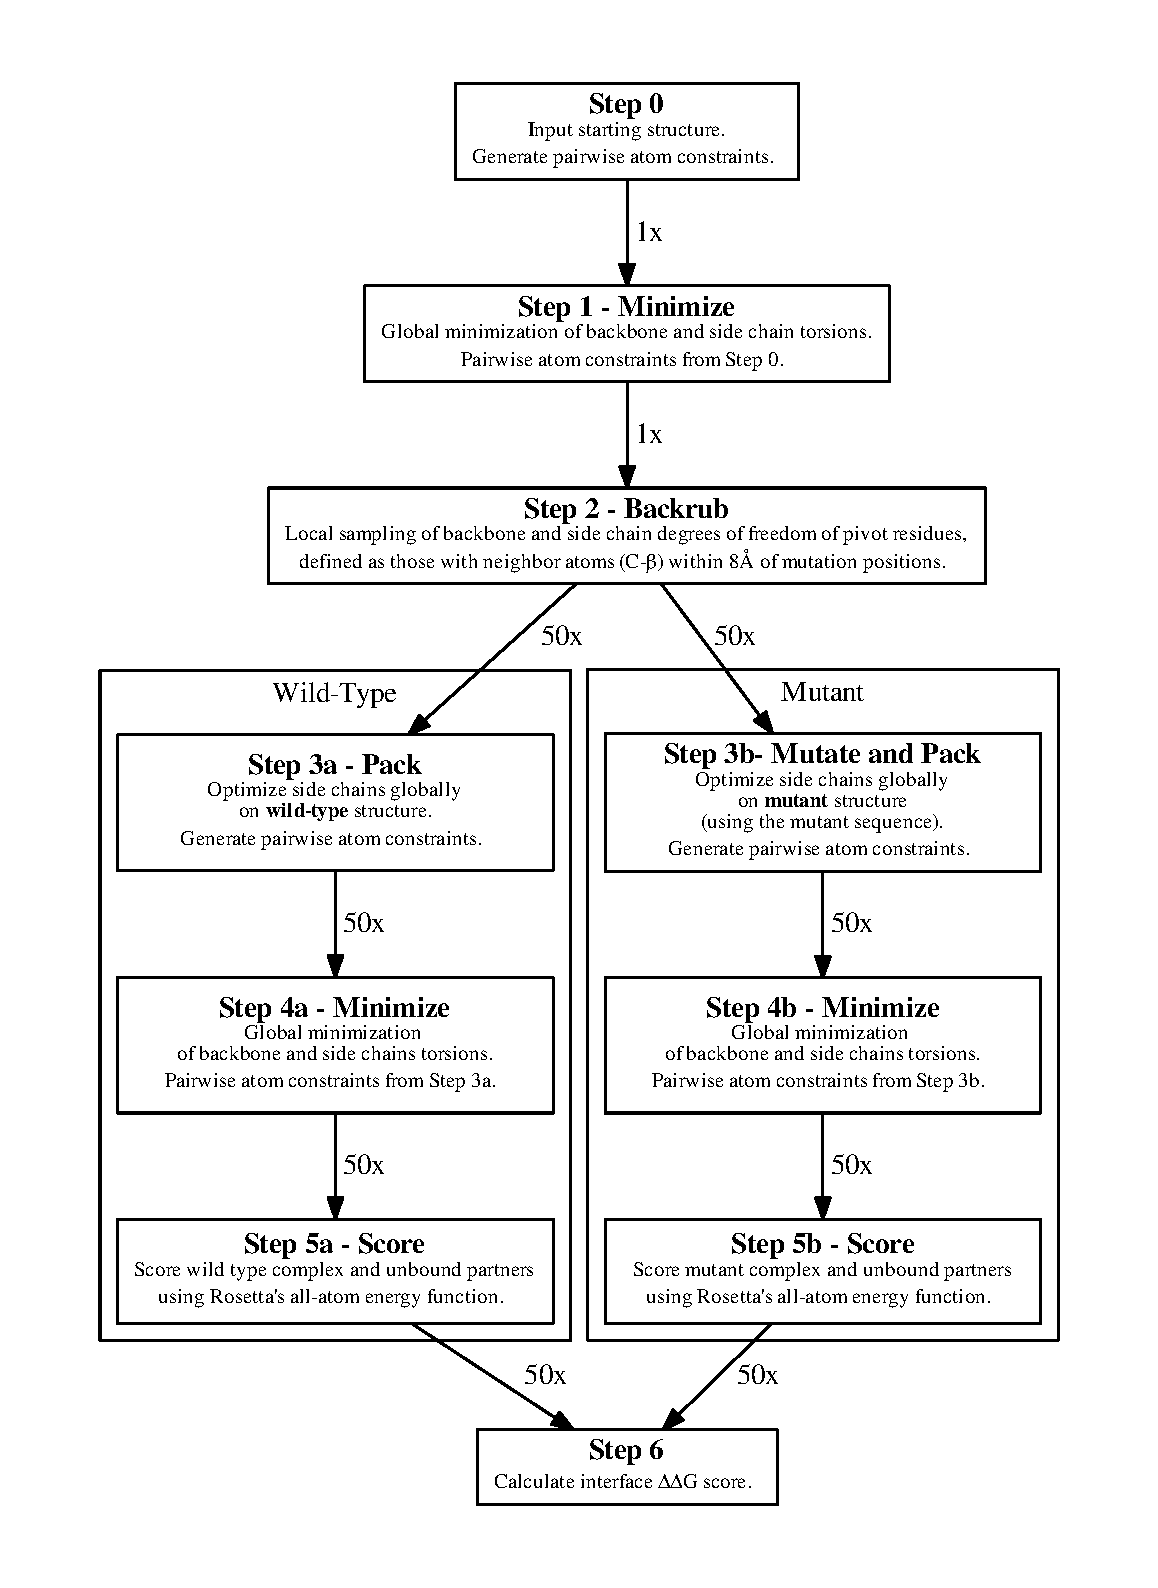
\includegraphics[width=\textwidth,keepaspectratio]{figures/fig-overview.pdf}
    \caption[]{
      Schematic of the flex ddG protocol method.
  } \label{fig:figure-overview}
\end{figure}

\subsection{Prediction protocol}

Flex ddG method steps are outlined in \cref{fig:figure-overview}. The method can be run using a Rosetta Scripts XML that is available in the Supporting Information as \cref{lst:ddg-script}.

\textbf{Step 1:} The protocol begins with an initial minimization (on backbone $\phi$/$\psi$\ and side chain $\chi$\ torsional degrees of freedom, using the ``lbfgs\_armijo\_nonmonotone'' minimization algorithm option) of the input model using the Rosetta energy function. This (and later) minimizations are performed with constraints that harmonically restrain pairwise atom distance to their values in the input crystal structure. Minimization is run until convergence (absolute score change upon minimization of less than one REU (Rosetta Energy Unit) is achieved.
\textbf{Step 2:} Starting from the minimized input structure, the backrub method in Rosetta\cite{smith_backrub-like_2008} is used to create an ensemble of models. In brief, each backrub move is undertaken on a randomly chosen protein segment consisting of three or more adjacent residues in the ``neighborhhood'' of any mutant position.
The mutation neighborhood is defined by finding all residues with a C-$\beta$ atom (C-$\alpha$ for glycines) within 8 \AA\ of any mutant position, then adding this residue and its adjacent N and C-terminal neighbors to the list of neighborhood residues.
All atoms in the three-residue segment are rotated locally about an axis defined as the vector between the endpoint C-$\alpha$ atoms. Backrub is run at a temperature of 1.2 kT, for up to 50,000 backrub Monte Carlo trials/steps (\cref{tab:table-temperature} shows that using a kT of 1.6 gives similar results to a kT of 1.2). Up to 50 output models are generated.
\textbf{Step 3A:} For each of the 50 models in the ensemble (output by backrub), the Rosetta ``packer'' is used to optimize side chain conformations for the wild-type sequence using discrete rotameric conformations \cite{shapovalov_smoothed_2011} and simulated annealing. The packer is run with the multi-cool annealer option\cite{leaver-fay_generic_2011}, which is set to keep a history of the 6 best rotameric states visited during annealing.
\textbf{Step 3B:} Independently and in parallel to step 3A, side chain conformations for the mutant sequence are optimized on all 50 models.
\textbf{Step 4A:} Each of the 50 wild-type models is minimized, again adding pairwise atom-atom constraints to the input structure. Minimization is run with the same parameters as in step 1; the coordinate constraints used in this step are taken from the coordinates of the Step 3A model.
\textbf{Step 4B:} As Step 4A, but for each of the 50 mutant models.
\textbf{Step 5A:} Each of the 50 minimized wild-type models are scored in complex, and the complex partners are scored individually. The scores of the split, unbound complex partners are obtained simply by moving the complex halves away from each other. No further minimization or side chain optimization is performed on the unbound partners before scoring.
\textbf{Step 5B:} In the same fashion as Step 5A, each of the 50 minimized mutant models are scored in complex, and the complex partners are scored individually.
\textbf{Step 6:} The interface \ddg\ score is produced via Eq. \ref{eqn:split-ddg}:

\begin{equation}\label{eqn:split-ddg}
  \begin{split}
    {\Delta\Delta}G_{bind} & ={\Delta}G^{MUT}_{bind} - {\Delta}G^{WT}_{bind}\\
    & =({\Delta}G^{MUT}_{complex} - {\Delta}G^{MUT}_{partner A} - {\Delta}G^{MUT}_{partner B})\\
    & \quad - ({\Delta}G^{WT}_{complex} - {\Delta}G^{WT}_{partner A} - {\Delta}G^{WT}_{partner B})\\
  \end{split}
\end{equation}

We evaluate performance of the protocol by comparing predicted \ddg\ scores to known experimental values, using Pearson's correlation (R), Fraction Correct (FC), and Mean Absolute Error (MAE). Fraction Correct is defined as the number of mutations categorized correctly as stabilizing, neutral, or destabilizing, divided by the total number of mutations in the benchmark set. Stabilizing mutations are defined as those with a \ddg\ $<=$\ -1.0 kcal/mol, neutral as those with -1.0 kcal/mol $<$\ \ddg\ $<$\ 1.0 kcal/mol, and destabilizing as those with \ddg\ $>=$\ 1.0 kcal/mol.

MAE (Mean Absolute Error) is defined in Eq.~\ref{eqn:mae} as:

\begin{equation}\label{eqn:mae}
  MAE = \dfrac{1}{n}\sum\limits_{i=1}^n|y_i-x_i| = \dfrac{1}{n}\sum\limits_{i=1}^n|e_i|
\end{equation}

where $y_i$ are the predicted \ddg\ values, $x_i$ are the known, experimentally determined values, and $e_i$ is the prediction error.

\subsection{Score analysis}

To investigate potential sources of prediction error on an individual score term basis, we used a generalized additive model\cite{hastie_generalized_1990} approach to fit Rosetta's predicted \ddg\ values to experimentally known values.
First, we apply an unbiased logistic scaling to individual score terms,
$$h_{a,b}(x) = \frac{e^{a}}{1 + \exp(- e^{b} x)},$$
where $a$ is the scaling range of the score, and $b$ is the steepness of the sigmoid scaling. Both parameters are transformed through an exponential to ensure non-negativity. The scaling function $h$ does not introduce bias, that is, $h_\theta(0) = 0$ for any $\theta$. The scoring model results in a generalized additive model (GAM) over the $M$ score terms,
$$f(\bf{x}) = \sum_{j=1}^M h_{a_i,b_i}(x).$$
The parameters $\theta = (a_j,b_j)_{j=1}^M$ for the score terms were simultaneously sampled using a random walk Metropolis-Hastings MCMC algorithm (the \texttt{mhsample} function in Matlab) assuming a Gaussian likelihood as the target distribution
$$p(\theta ; \bf{y}) = N( f(\bf{x}_i) | y_i, \sigma_n^2)$$
with a noise variance set to $\sigma_n^2 = 1.0$, and where $(\bf{x}_i,y_i)_{i=1}^N$ are the empirical observations $y_i$ that correspond to the protein score terms $\bf{x}_i$, respectively. We sample for $1000$ samples with a burn-in set to $1000$ samples and a thinning parameter of $20$. The proposal distribution was selected to be a symmetric uniform distribution such that $[a^{(s+1)},b^{(s+1)}] \sim U( a^{(s)} \pm 2, b^{(s)} \pm 2)$. The resulting MCMC sample represents all logistics score scalings that reproduce the empirical measurements assuming an error model with noise variance $\sigma_n^2$.

\section{Results and discussion}

\subimport*{figs-and-tables/}{table-main}

The overall performance of the protocol is summarized in \cref{tab:table-main}.
We compare 4 prediction methods: (a) our flex ddG backrub ensemble method, (b) the prior state-of-the-art Rosetta methodology, ddg\_monomer \cite{kellogg_role_2011}, (c) a control version of our flex ddG protocol which omits the backrub ensemble generation step, leaving only the minimization and packing steps, and (d) published data from the ZEMu (zone equilibration of mutants) method\cite{dourado_multiscale_2014}. Data split by input protein-protein complex are shown in \cref{tab:table-by-structure}.

The new flex ddG method outperforms the comparison methods on the complete dataset in each of the correlation, MAE, and fraction correct metrics (Table 2). In particular, we see a large increase in performance relative to the other methods on the small-to-large subset of mutations. This is in accordance with our expectations that backrub ensembles should be able to sample small backbone conformational adjustments required to accommodate changes in amino acid residue size. Notably, application of backrub ensembles performs better than other methods that include backbone minimization steps only, including the current state-of-the-art Rosetta ddg\_monomer method. On the small-to-large mutations subset, the ddg\_monomer method achieves a Pearson correlation of only 0.31 compared to 0.64 with flex ddg.

Performance of the flex ddG on the subset of single mutations to alanine is also competitive or outperforms the alternative methods.
As we do not expect single mutations to alanine to require intensive backbone sampling, our method's effectiveness on this subset shows that the method is fairly robust to the mutation type.
As we chose to perform backrub sampling prior to introducing mutations, these results suggest that flex ddG is effective by sampling underlying, relevant plasticity of the input crystal structure instead of distorting the local structure around a mutation to resolve a clash or poor interaction with a mutant side chain.

The flex ddg method also shows improved performance compared to the control method and ddg\_monomer on the subset of multiple mutations, but for this set does not match the performance of the ZEMu method.
This result could indicate that further refinement to the backrub sampling parameters is required when simultaneously sampling conformational space around the sites of multiple mutations.
However and remarkably, flex ddG outperforms ZEMu on a subset of cases with multiple mutations where none of the mutations are to alanine (\cref{tab:table-main}). Finally, the flex ddg method also shows considerable improvements over other methods on the subset of antibody-antigen complexes (Table 2).

\cref{fig:figure-scatter} illustrates the performance for the flex ddG and control methods on the complete dataset and small-to-large subsets using scatterplots comparing experimentally determined and computationally estimated changes in binding free energies for each of the cases in the datasets. In particular, a notable improvement with flex ddG over the control can be seen for the 13 small-to-large mutations that were experimentally determined to stabilize the protein-protein interface significantly (\ddg\ $<=$\ -1.0 kcal/mol). For this set, the control method misclassifies most stabilizing mutations to have minimal effect or to be destabilizing (9 mutations with predicted Rosetta \ddg\ scores $>$\ 0) (\cref{fig:figure-scatter}d), whereas flex ddG identifies a sizeable number (12 of 13 mutations) to have predicted Rosetta $\Delta\Delta G < 0$ (\cref{fig:figure-scatter}c), even though only 1 of these mutations is predicted to be strongly stabilizing (predicted \ddg\ score < 1). The capability to predict stabilizing mutations is especially important for challenging design applications to modulate binding affinity as well as selectivity, as well as creating entirely new high-affinity protein-protein interactions.

In the following sections, we assess how different flex ddG implementations would affect its prediction performance, focusing separately on sampling and scoring.

\subimport*{figs-and-tables/}{figure-scatter}

\subimport*{figs-and-tables/}{structs-v-corr-WildTypeComplex-zemu-12-60000-rscript-simplified-t14}

\subsection{Effect of ensemble size}

The results presented above used an ensemble size of 50 members but it is unclear what the optimal ensemble size should be. For example, prior methods used ensemble sizes ranging from ten\cite{kamisetty_accounting_2011}\ to thousands\cite{benedix_predicting_2009}. As here the computational time increases linearly with ensemble size, determining an optimal size is practically relevant. We therefore evaluated the performance of flex ddG as we average across an increasing number of models (from 1 to 50, \cref{fig:structs-v-corr-WildTypeComplex-zemu-12-60000-rscript-simplified-t14}.
The models are first sorted by the score of the corresponding repacked and minimized wild type model, such that producing a \ddg\ with 1 model will only use the lowest (best) scoring model, 2 models will use the 2 lowest scoring models, and so forth.
\cref{fig:structs-v-corr-WildTypeComplex-zemu-12-60000-rscript-simplified-t14}(a) shows the performance on the complete dataset.
As more models with increasing wild type complex score are averaged, correlation with known experimental values increases.
Conversely, performance for the no backrub control method stays approximately constant as more models are averaged.
This result indicates that sampling with backrub adds information that improves \ddg\ calculation even though the additional averaged models have higher scores (average ensemble total score is shown in \cref{fig:wildtypecomplex-scores-complete}).
These higher scoring models would typically be excluded in methods such as the Rosetta ddg\_monomer protocol, which uses only the single lowest scoring wild-type and mutant models.

Instead of using just the three lowest energy models\cite{kellogg_role_2011}, we find that the performance of the ddg\_monomer method also improves as more output models are averaged (\cref{fig:structs-v-corr-WildTypeComplex-ddg-monomer-16-003-zemu-2}, \cref{tab:structs-v-corr-WildTypeComplex-ddg-monomer-16-003-zemu-2-underlying-data}).
This was somewhat unexpected, as the no-backrub control method, which did not show an improvement with increasing ensemble size, is conceptually similar to the ddg\_monomer method. However, the difference may arise from the fact that the ddg\_monomer method ramps the repulsive term of the energy function during minimization. This strategy explores conformational space more broadly in different backbone ensemble members than minimization with a fully weighted repulsive term in the no-backrub control method. In this fashion, including more ensemble members generated by the ddg\_monomer method increases the conformational plasticity sampled which in turn increases performance, as seen for the flex ddg method.

The subset of small-to-large mutations shows the largest increase in correlation with experimental \ddg\ values as more models are averaged (\cref{fig:structs-v-corr-WildTypeComplex-zemu-12-60000-rscript-simplified-t14}(b)). This result is consistent with our reasoning above that improved modeling of conformational plasticity is important for prediction performance, and that this effect is most important for significant changes in amino acid residue size. For the subset of multiple mutations where none are mutations to alanine (\cref{fig:structs-v-corr-WildTypeComplex-zemu-12-60000-rscript-simplified-t14}(c)), performance fluctuates with fewer models, but shows a robust increase when more than about 12 models are averaged. This observation indicates modeling limitations in particular where sampling of larger regions might be necessary for multiple mutations.

Averaging across increased numbers of models also improves correlation for the subset of single mutations to alanines (\cref{fig:structs-v-corr-WildTypeComplex-zemu-12-60000-rscript-simplified-t14}(d)).
Here, improvements are seen up to averaging about 10 models, after which performance stays approximately constant.
This observation indicates that increased sampling, in the very least, is not harmful for cases where one would expect structural changes to be relatively small on average.

From a practical standpoint, simply generating 20-30 models should constitute sufficient sampling for most cases. Sorting the generated models by score and selecting the best scoring 20 out of 50 models does not appear to be necessary, as not sorting the models by score (\cref{fig:structs-v-corr-id-zemu-12-60000-rscript-simplified-t14}, \cref{tab:structs-v-corr-id-zemu-12-60000-rscript-simplified-t14-underlying-data}) gives similar results to sorting the models (\cref{fig:structs-v-corr-WildTypeComplex-zemu-12-60000-rscript-simplified-t14}).

\subsection{Effect of extent of backrub sampling in each trajectory}

\subimport*{figs-and-tables/}{steps-v-corr}

The extent of sampling can also be controlled by changing the number of Monte Carlo steps in the backrub simulations.
\cref{fig:steps-v-corr} shows the effect of increasing the number of backrub Monte Carlo steps (while averaging all 50 models at each output step) on flex ddG performance, compared to a control method with zero backrub steps that uses only minimization and side chain packing.
\ddg\ scores are calculated every 2,500 backrub steps.

After an initial increase for the first set of 2500 backrub steps, performance stays relatively constant for the complete dataset (Figure 4a) and for single mutations to alanine (\cref{fig:steps-v-corr}d). However, for the subsets of small-to-large mutations (Figure 4b) and multiple mutations, none to alanine (\cref{fig:steps-v-corr}c), performance increases considerably with increasing numbers of Monte Carlo steps. This increase in performance is similar to what we observed with averaging over more models for these subsets (\cref{fig:structs-v-corr-WildTypeComplex-zemu-12-60000-rscript-simplified-t14}b,c).
Performance reaches a maximum at around 30,000 backrub Monte Carlo steps, after which it levels off.

The increased performance does not appear to be simply a result of decreasing scores as the simulation progresses, as the average score of the minimized wild type complexes does not decrease uniformly across the sampled ensemble as the simulation progresses (\cref{fig:wildtypecomplex-scores-complete}).
The pairwise backrub ensemble RMSDs continue to increase throughout the backrub simulation for all subsets (\cref{fig:t14-mean-ensemble}), indicating that diminishing returns at > 30,000 Monte Carlo steps is not a result of failure to sample new conformations, but rather might indicate that continued sampling does not capture additional relevant local changes in structure that occur post-mutation in this benchmark set.

\subsection{Score analysis}

As the sampling/scoring problems of protein modeling are generally linked, it is often the case that improving one enables further improvements on the other.

First, we compared the performance of our flex ddG method, which was run using Rosetta's Talaris\cite{song_structure-guided_2011,shapovalov_smoothed_2011,omeara_combined_2015} energy function, to an identical protocol run with the more recently developed Rosetta Energy Function (REF)\cite{alford_rosetta_2017}. We did not observe an increase in performance on the complete ZEMu dataset, and performance decreases were seen for the subsets of small-to-large mutations and multiple mutations (\cref{tab:table-ref}). Interestingly, flex ddG performance with the REF energy function increased over using the Talaris energy function if the resolution of the input crystal structure was $<= 1.5 \AA$, but this subset of the data was rather small with only 52 mutations.

Next, we sought to analyze underlying errors of the Rosetta energy function (when applied to interface \ddg) by assessing the individual terms of the energy function. To do so, we chose to reweight the terms of the energy function using a non-linear reweighting scheme similar to Generalized Additive Models (GAMs)\cite{hastie_generalized_1990}.
In this reweighting method, we use Monte Carlo sampling to fit a sigmoid function to the individual distributions of energy function terms, with the objective function of reducing the absolute error between our predictions and known experimental values over the entire dataset.

\begin{figure}
  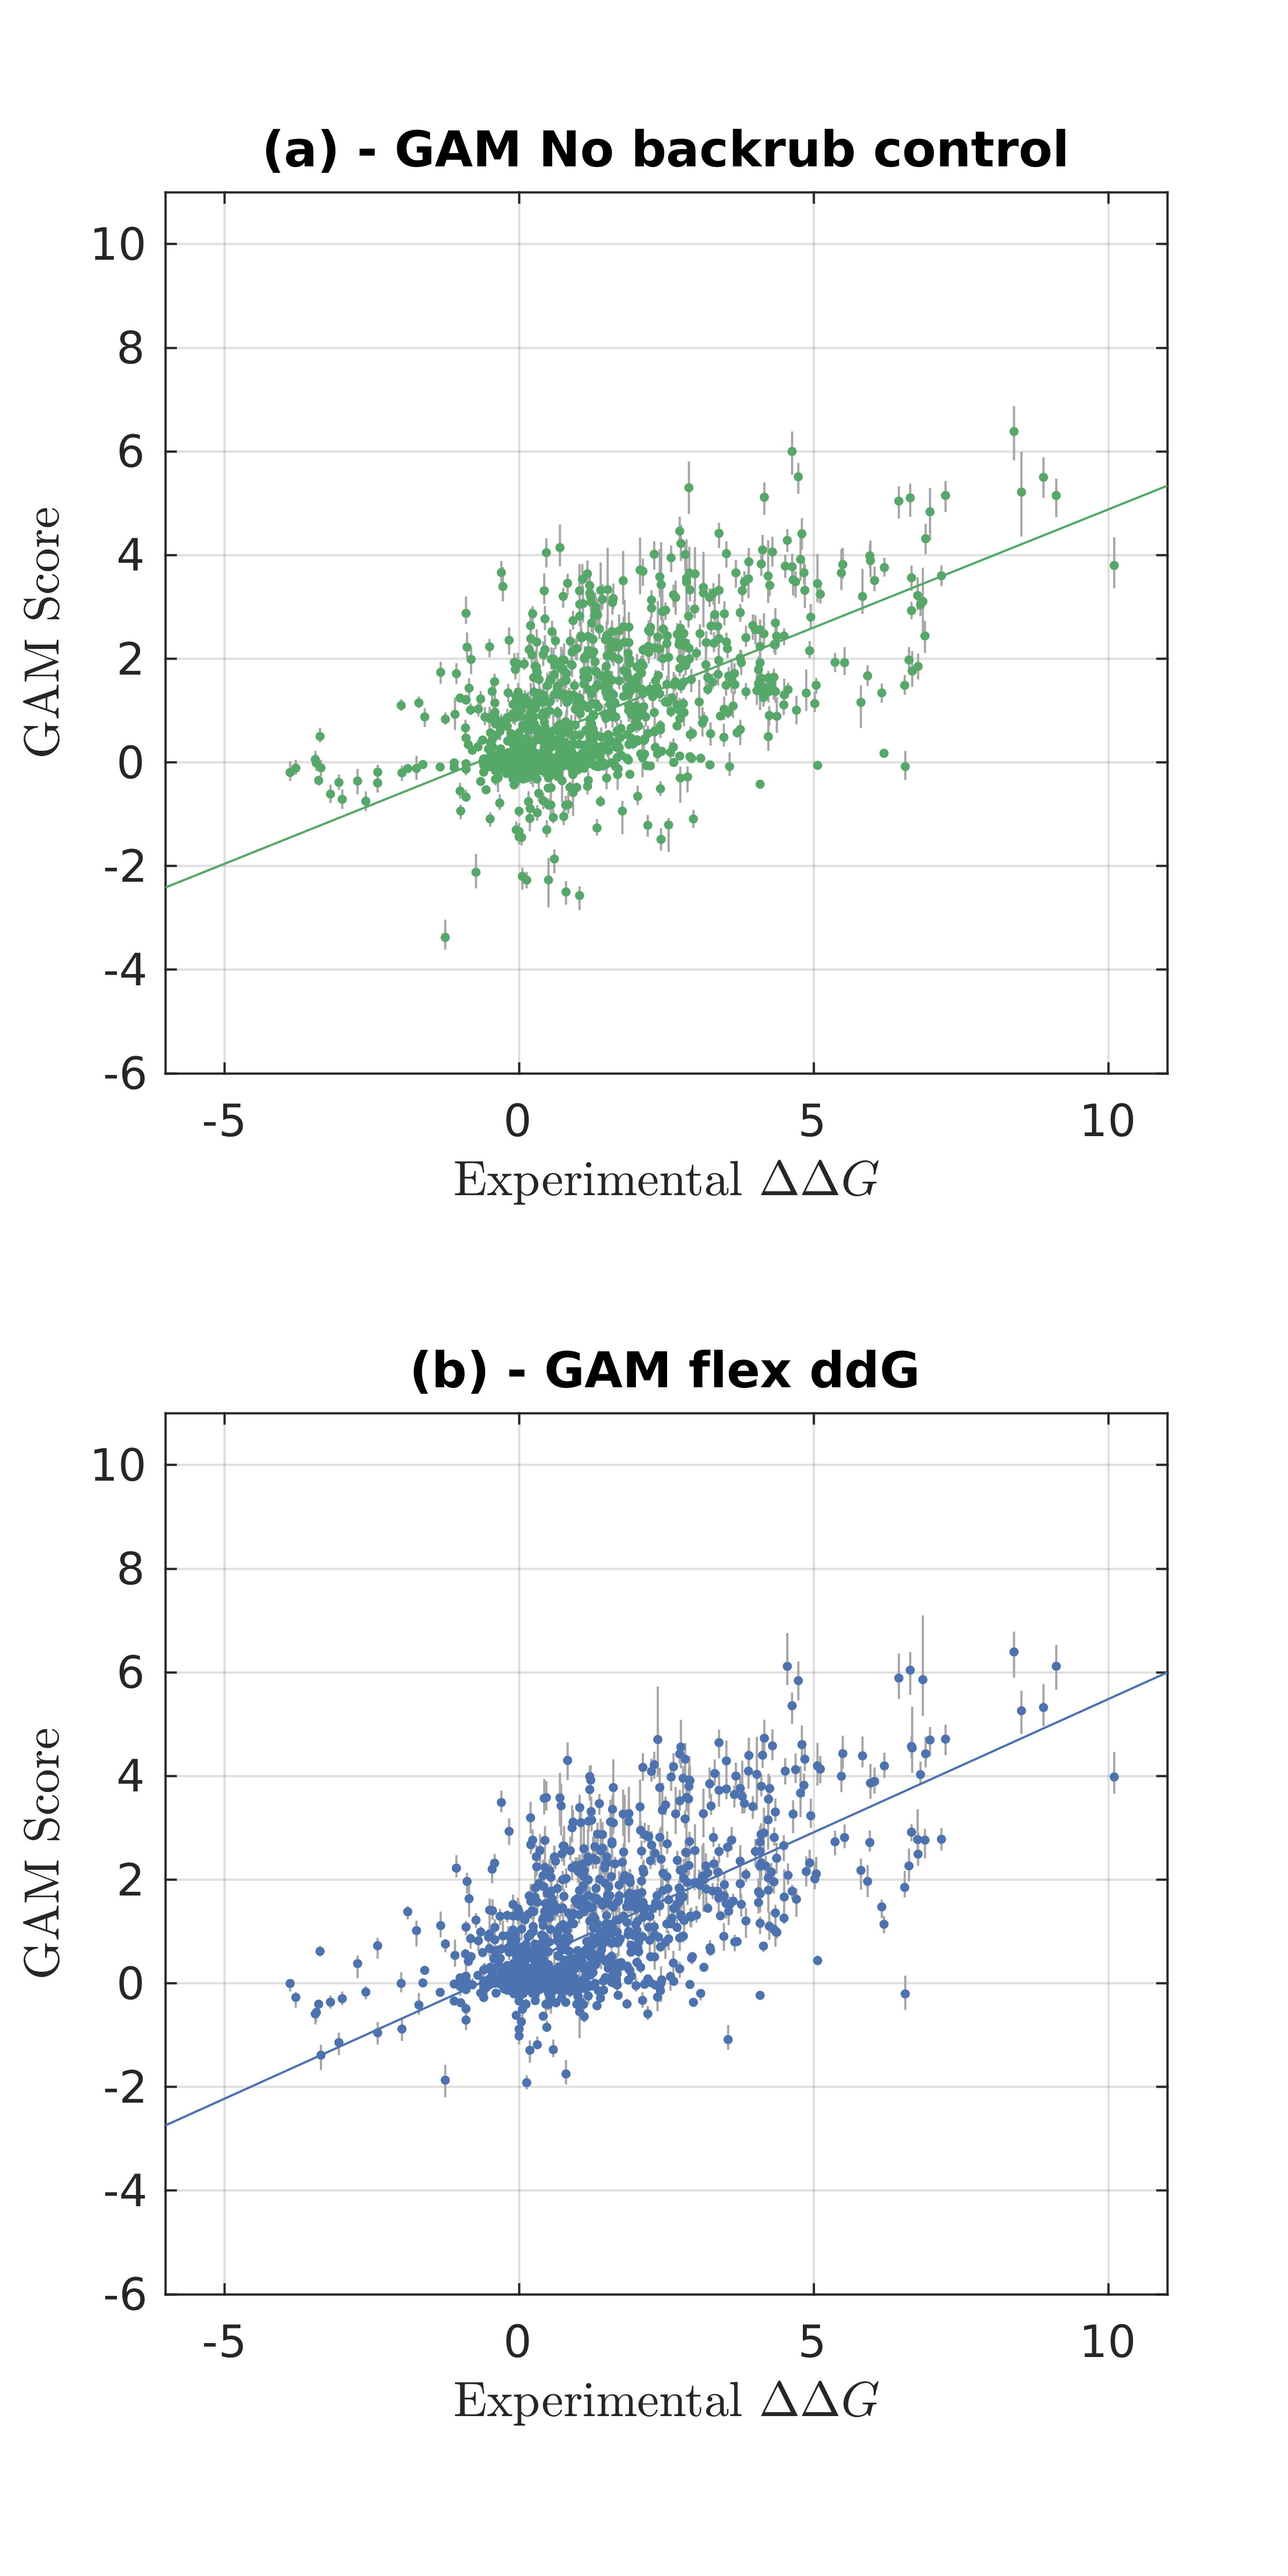
\includegraphics[width=0.5\textwidth,keepaspectratio]{figures/zemu-sigmoid2-corrs-main.png}
  \caption[]{
    Experimentally determined $\Delta\Delta G$ values (x-axis) versus predictions using a Generalized additive model (GAM).
    GAM scores are refit from values in Rosetta Energy Units (REU) using the Rosetta Talaris\cite{song_structure-guided_2011,shapovalov_smoothed_2011,omeara_combined_2015} energy function.
    The error bars in gray represent the range from minimum to maximum fit predicted \ddg\ value for the 1000 sampled GAM models.
    \textbf{(a)}: Control (no backrub) Rosetta predictions.
    \textbf{(b)}: Flex ddG Rosetta predictions using 35,000 backrub steps and 50 output models.
    A line of best fit is shown in each of the panels.
  } \label{fig:t14-fit-scatter-main}
\end{figure}

The effect on the predictions is shown in \cref{fig:t14-fit-scatter-main}, \cref{fig:t14-fit-scatter-supp}, and \cref{tab:table-gam-fit}. In general, the GAM-adjusted predictions contain fewer outliers. In particular, experimental \ddg\ values that are relatively neutral (near zero) can sometimes be predicted by flex ddG to be highly destabilizing; the GAM model reduces the magnitude of error of many of these outliers, improving overall performance. The overall correlation increases from 0.64 to 0.68 when refitting the values from the Rosetta Talaris energy function\cite{song_structure-guided_2011,shapovalov_smoothed_2011,omeara_combined_2015}; refitting values from the Rosetta REF energy function\cite{alford_rosetta_2017} leads to a similar increase from 0.63 to 0.68 (Fig. S6). The correlation coefficient also increases when refitting the values obtained for the no backrub control, but only to 0.62 (Fig. 5b)

The fit functions (fit for Talaris-derived \ddg\ predictions) are shown in \cref{fig:t14-fits-feats}. Extreme values for most score terms are downweighted, especially for the fa\_sol and fa\_atr terms, which make the largest contributions to predicted \ddg\ (\cref{fig:tal-GAM-terms-mpl}).

\section{Conclusions}

We have shown on a large, curated benchmark dataset that the ``flex ddG'' method presented here is more accurate than previous methods for estimating changes in binding affinity after mutation in protein-protein interfaces.
Particular improvement in performance is seen on the subset of small-to-large mutations, indicating that representing backbone flexibility using backrub motions is effective in cases where backbone rearrangements are expected to be more common. Other notable improvements over previous methods are seen for stabilizing mutations, mutations in antibody-antigen interfaces, and for cases with multiple changes where none of the mutations is to an alanine residue.

We have also shown that more accurate predictions can be obtained by averaging the predictions across a generated structural ensemble of backrub models, and that the number of required models is relatively low (20-30).
Prior methods that produced \ddg\ predictions by averaging an ensemble of models required on the order of thousands of models  \cite{benedix_predicting_2009}, indicating that backrub sampling can efficiently sample the local conformational landscape around an input wild-type structure that is relevant for interface \ddg\ prediction.

By creating a method that uses backrub to sample conformational space more broadly than minimization alone, while still staying close to the known wild-type input structure, we have also generated data that should prove useful for future energy function improvements.
In particular, performance with Rosetta's newest REF energy function\cite{alford_rosetta_2017} is currently not better in our method than performance with the prior Talaris\cite{leaver-fay_chapter_2013,song_structure-guided_2011,shapovalov_smoothed_2011} energy function (\cref{tab:table-ref}), indicating that the backrub sampling parameters might require further benchmarking and adaption to the REF energy function.
Our error analysis via GAM-like reweighting also indicates potential avenues for energy function improvement by identifying imbalances in predicted energetic contributions leading to overestimation of stabilizing and destabilizing effects.
Further improvements might also be obtained by more explicitly including the effects of altering water-mediated interactions\cite{lai_enhancing_2017} and of conformational entropy\cite{hu_protein_2006,guerois_predicting_2002}, as well as by considering the commonly observed shortcomings of energy functions balancing the magnitudes of electrostatic interactions and desolvation costs.
We expect energy function improvements to require more accurate representation of subtler conformational changes, as these changes can have a considerable impact on design predictions\cite{dou_sampling_2017}.

%%%%%%%%%%%%%%%%%%%%%%%%%%%%%%%%%%%%%%%%%%%%%%%%%%%%%%%%%%%%%%%%%%%%%
%% The "Acknowledgement" section can be given in all manuscript
%% classes.  This should be given within the "acknowledgement"
%% environment, which will make the correct section or running title.
%%%%%%%%%%%%%%%%%%%%%%%%%%%%%%%%%%%%%%%%%%%%%%%%%%%%%%%%%%%%%%%%%%%%%
\begin{acknowledgement}
  The authors acknowledge the following sources of funding:
T.K. was supported by grants from the National Institute of Health (R01 GM110089 and R01 GM117189). T.K. is a Chan Zuckerberg Biohub investigator.
M.H. was supported by Academy of Finland grant 299915.
S.T. and J.E.L. were supported by National Science Foundation Graduate Research Fellowships.
% TODO add new
\end{acknowledgement}

%%%%%%%%%%%%%%%%%%%%%%%%%%%%%%%%%%%%%%%%%%%%%%%%%%%%%%%%%%%%%%%%%%%%%
%% The same is true for Supporting Information, which should use the
%% suppinfo environment.
%%%%%%%%%%%%%%%%%%%%%%%%%%%%%%%%%%%%%%%%%%%%%%%%%%%%%%%%%%%%%%%%%%%%%
\begin{suppinfo}
\documentclass[journal=jpcbfk,manuscript=suppinfo]{achemso}
\setkeys{acs}{doi = true}

\usepackage[T1]{fontenc}       % Use modern font encodings
\usepackage[capitalise]{cleveref}
\usepackage{import}
\usepackage{booktabs}
\usepackage{multirow}
\usepackage{csvsimple}
\usepackage{longtable}
\usepackage{graphicx}
\usepackage{listings}
\usepackage{minted}
\usepackage{caption}
\usepackage{pdflscape}

\newcommand\ddg{$\Delta\Delta G$}

\usepackage{xr} % Probably not needed for submission
\externaldocument{flex-ddG}

%%%%%%%%%%%%%%%%%%%%%%%%%%%%%%%%%%%%%%%%%%%%%%%%%%%%%%%%%%%%%%%%%%%%%
%% Meta-data block
%% ---------------
%% Each author should be given as a separate \author command.
%%
%% Corresponding authors should have an e-mail given after the author
%% name as an \email command. Phone and fax numbers can be given
%% using \phone and \fax, respectively; this information is optional.
%%
%% The affiliation of authors is given after the authors; each
%% \affiliation command applies to all preceding authors not already
%% assigned an affiliation.
%%
%% The affiliation takes an option argument for the short name.  This
%% will typically be something like "University of Somewhere".
%%
%% The \altaffiliation macro should be used for new address, etc.
%% On the other hand, \alsoaffiliation is used on a per author basis
%% when authors are associated with multiple institutions.
%%%%%%%%%%%%%%%%%%%%%%%%%%%%%%%%%%%%%%%%%%%%%%%%%%%%%%%%%%%%%%%%%%%%%
\author{Kyle A. Barlow}
\affiliation{Graduate Program in Bioinformatics, University of California San Francisco, San Francisco, California, United States of America}
\email{kb@kylebarlow.com}
\author{Other Authors To Be Added}
\affiliation{Graduate Program in Bioinformatics, University of California San Francisco, San Francisco, California, United States of America}
\author{Tanja Kortemme}
\affiliation[QB3]{California Institute for Quantitative Biosciences, University of California San Francisco, San Francisco, California, United States of America}
\alsoaffiliation{Department of Bioengineering and Therapeutic Sciences, University of California San Francisco, San Francisco, California, United States of America}
\alsoaffiliation{Graduate Program in Bioinformatics, University of California San Francisco, San Francisco, California, United States of America}
\alsoaffiliation{Graduate Program in Biophysics, University of California San Francisco, San Francisco, California, United States of America}
\email{kortemme@cgl.ucsf.edu}

%%%%%%%%%%%%%%%%%%%%%%%%%%%%%%%%%%%%%%%%%%%%%%%%%%%%%%%%%%%%%%%%%%%%%
%% The document title should be given as usual. Some journals require
%% a running title from the author: this should be supplied as an
%% optional argument to \title.
%%%%%%%%%%%%%%%%%%%%%%%%%%%%%%%%%%%%%%%%%%%%%%%%%%%%%%%%%%%%%%%%%%%%%
\title[]
  {Flex ddG: Rosetta ensemble-based estimation of changes in protein-protein binding affinity upon mutation}

% A listing of the contents of each file supplied as Supporting Information
% should be included. For instructions on what should be included in the
% Supporting Information as well as how to prepare this material for
% publications, refer to the journal's Instructions for Authors.

% The following files are available free of charge.
% \begin{itemize}
% \item Filename: brief description
% \item Filename: brief description
% \end{itemize}

% Supplementary figures:
% \begin{itemize}
% \item \cref{tab:table-mult}
% \item \cref{fig:steps-v-corr}
% \item \cref{tab:table-versions}
% \item \cref{fig:structs-v-corr-id-zemu-12-60000-rscript-simplified-t14}
% \item \cref{fig:structs-v-corr-WildTypeComplex-ddg-monomer-16-003-zemu-2}
% \item \cref{fig:wildtypecomplex-scores-complete}
% \item \cref{fig:spear-corr-rmsd-error}
% \item \cref{fig:t14-mean-ensemble}
% \item \cref{tab:table-ref}
% \item \cref{tab:table-antibodies}
% \item \cref{fig:t14-fits-feats}
% \end{itemize}

\begin{document}

\renewcommand{\thefigure}{S\arabic{figure}}
\setcounter{figure}{0}
\renewcommand{\thetable}{S\arabic{table}}
\setcounter{table}{0}
% \renewcommand{\lstlistingname}{Code Listing}
\renewcommand*{\thepage}{S\arabic{page}}

\subimport*{figs-and-tables/}{table-versions}
\subimport*{figs-and-tables/}{table-temperature}
\clearpage
{\small
\begin{longtable}{llrrrr}
\toprule
Mutation Category &   Prediction Method &   N &     R &  MAE &   FC \\
\midrule
 \multirow{ 4}{*}{pdb-1A22} & flex ddG & \multirow{ 4}{*}{142} & \textbf{0.32} & \textbf{0.61} & \textbf{0.79}  \\
 & no backrub control & & 0.18 & 0.77 & 0.74  \\
 & ddG monomer & & 0.12 & 0.91 & 0.73  \\
 & ZEMu paper & & 0.19 & 0.68 & 0.78  \\
\hline
 \multirow{ 4}{*}{pdb-1A4Y} & flex ddG & \multirow{ 4}{*}{45} & 0.81 & 1.34 & 0.71  \\
 & no backrub control & & 0.79 & 1.47 & \textbf{0.78}  \\
 & ddG monomer & & 0.77 & 1.91 & 0.62  \\
 & ZEMu paper & & \textbf{0.87} & \textbf{1.12} & 0.73  \\
\hline
 \multirow{ 4}{*}{pdb-1ACB} & flex ddG & \multirow{ 4}{*}{6} & 0.28 & 2.89 & 0.83  \\
 & no backrub control & & 0.23 & 2.37 & 0.83  \\
 & ddG monomer & & 0.58 & \textbf{1.57} & \textbf{1.00}  \\
 & ZEMu paper & & \textbf{0.79} & 2.17 & 0.83  \\
\hline
 \multirow{ 4}{*}{pdb-1AHW} & flex ddG & \multirow{ 4}{*}{10} & -0.83 & 1.31 & 0.4  \\
 & no backrub control & & -0.42 & 1.42 & 0.4  \\
 & ddG monomer & & -0.34 & 1.26 & 0.5  \\
 & ZEMu paper & & \textbf{0.30} & \textbf{0.93} & \textbf{0.6}  \\
\hline
 \multirow{ 4}{*}{pdb-1AK4} & flex ddG & \multirow{ 4}{*}{15} & \textbf{0.73} & \textbf{0.53} & \textbf{0.73}  \\
 & no backrub control & & 0.35 & 1.01 & 0.47  \\
 & ddG monomer & & 0.63 & 1.35 & 0.60  \\
 & ZEMu paper & & 0.44 & 1.63 & 0.53  \\
\hline
 \multirow{ 4}{*}{pdb-1CBW} & flex ddG & \multirow{ 4}{*}{15} & 0.01 & \textbf{0.59} & \textbf{0.87}  \\
 & no backrub control & & \textbf{0.05} & 0.83 & 0.67  \\
 & ddG monomer & & -0.09 & 0.72 & 0.67  \\
 & ZEMu paper & & -0.26 & 0.71 & 0.67  \\
\hline
 \multirow{ 4}{*}{pdb-1CSE} & flex ddG & \multirow{ 4}{*}{6} & 0.44 & 1.94 & 0.67  \\
 & no backrub control & & 0.37 & 2.03 & 0.67  \\
 & ddG monomer & & 0.46 & 1.88 & 0.67  \\
 & ZEMu paper & & \textbf{0.87} & \textbf{0.81} & \textbf{1.00}  \\
\hline
 \multirow{ 4}{*}{pdb-1DAN} & flex ddG & \multirow{ 4}{*}{118} & 0.65 & \textbf{0.53} & \textbf{0.88}  \\
 & no backrub control & & \textbf{0.69} & 0.59 & 0.85  \\
 & ddG monomer & & 0.61 & 0.71 & 0.83  \\
 & ZEMu paper & & 0.32 & 0.88 & 0.76  \\
\hline
 \multirow{ 4}{*}{pdb-1DFJ} & flex ddG & \multirow{ 4}{*}{20} & 0.70 & 1.35 & \textbf{0.70}  \\
 & no backrub control & & \textbf{0.83} & \textbf{1.04} & 0.60  \\
 & ddG monomer & & 0.69 & 1.38 & 0.55  \\
 & ZEMu paper & & 0.55 & 1.40 & 0.55  \\
\hline
 \multirow{ 4}{*}{pdb-1DQJ} & flex ddG & \multirow{ 4}{*}{34} & \textbf{0.44} & \textbf{1.67} & 0.79  \\
 & no backrub control & & 0.39 & 1.93 & 0.65  \\
 & ddG monomer & & 0.37 & 1.87 & \textbf{0.82}  \\
 & ZEMu paper & & 0.28 & 2.08 & 0.59  \\
\hline
 \multirow{ 4}{*}{pdb-1DVF} & flex ddG & \multirow{ 4}{*}{38} & 0.63 & 1.58 & 0.53  \\
 & no backrub control & & \textbf{0.65} & \textbf{1.50} & 0.66  \\
 & ddG monomer & & 0.61 & 1.54 & \textbf{0.71}  \\
 & ZEMu paper & & 0.57 & 1.54 & 0.53  \\
\hline
 \multirow{ 4}{*}{pdb-1E96} & flex ddG & \multirow{ 4}{*}{6} & \textbf{0.52} & \textbf{0.84} & 0.50  \\
 & no backrub control & & 0.51 & 0.91 & 0.50  \\
 & ddG monomer & & 0.45 & 0.96 & 0.50  \\
 & ZEMu paper & & 0.50 & 0.85 & \textbf{0.67}  \\
\hline
 \multirow{ 4}{*}{pdb-1EAW} & flex ddG & \multirow{ 4}{*}{27} & 0.03 & 0.58 & 0.85  \\
 & no backrub control & & 0.07 & 0.73 & 0.81  \\
 & ddG monomer & & \textbf{0.13} & 0.61 & 0.89  \\
 & ZEMu paper & & 0.00 & \textbf{0.49} & \textbf{0.93}  \\
\hline
 \multirow{ 4}{*}{pdb-1EMV} & flex ddG & \multirow{ 4}{*}{51} & \textbf{0.89} & \textbf{0.86} & \textbf{0.86}  \\
 & no backrub control & & 0.84 & 0.98 & 0.84  \\
 & ddG monomer & & 0.84 & 0.96 & 0.80  \\
 & ZEMu paper & & 0.87 & 0.89 & 0.84  \\
\hline
 \multirow{ 4}{*}{pdb-1F47} & flex ddG & \multirow{ 4}{*}{12} & 0.56 & \textbf{0.72} & 0.50  \\
 & no backrub control & & 0.58 & 0.87 & \textbf{0.58}  \\
 & ddG monomer & & \textbf{0.60} & 0.87 & \textbf{0.58}  \\
 & ZEMu paper & & 0.51 & 1.02 & 0.42  \\
\hline
 \multirow{ 4}{*}{pdb-1FC2} & flex ddG & \multirow{ 4}{*}{9} & -0.07 & \textbf{0.84} & 0.56  \\
 & no backrub control & & -0.09 & 1.01 & 0.67  \\
 & ddG monomer & & -0.39 & 1.19 & 0.44  \\
 & ZEMu paper & & \textbf{0.28} & 0.89 & \textbf{0.78}  \\
\hline
 \multirow{ 4}{*}{pdb-1FCC} & flex ddG & \multirow{ 4}{*}{8} & -0.21 & 1.56 & \textbf{0.5}  \\
 & no backrub control & & -0.22 & 1.96 & \textbf{0.5}  \\
 & ddG monomer & & -0.06 & 1.50 & \textbf{0.5}  \\
 & ZEMu paper & & \textbf{0.16} & \textbf{1.35} & \textbf{0.5}  \\
\hline
 \multirow{ 4}{*}{pdb-1GC1} & flex ddG & \multirow{ 4}{*}{56} & 0.12 & \textbf{0.35} & \textbf{0.91}  \\
 & no backrub control & & -0.15 & 0.43 & 0.86  \\
 & ddG monomer & & 0.28 & 0.38 & 0.86  \\
 & ZEMu paper & & \textbf{0.36} & 0.55 & 0.84  \\
\hline
 \multirow{ 4}{*}{pdb-1HE8} & flex ddG & \multirow{ 4}{*}{10} & 0.39 & 0.67 & \textbf{0.5}  \\
 & no backrub control & & 0.62 & 0.91 & \textbf{0.5}  \\
 & ddG monomer & & 0.26 & \textbf{0.66} & 0.3  \\
 & ZEMu paper & & \textbf{0.81} & 1.23 & \textbf{0.5}  \\
\hline
 \multirow{ 4}{*}{pdb-1IAR} & flex ddG & \multirow{ 4}{*}{36} & 0.64 & \textbf{0.72} & 0.78  \\
 & no backrub control & & 0.35 & 1.32 & 0.67  \\
 & ddG monomer & & \textbf{0.66} & 0.98 & \textbf{0.81}  \\
 & ZEMu paper & & 0.45 & 0.86 & 0.78  \\
\hline
 \multirow{ 4}{*}{pdb-1JCK} & flex ddG & \multirow{ 4}{*}{7} & 0.46 & 1.22 & 0.57  \\
 & no backrub control & & 0.44 & 0.97 & \textbf{0.71}  \\
 & ddG monomer & & 0.75 & 1.25 & \textbf{0.71}  \\
 & ZEMu paper & & \textbf{0.85} & \textbf{0.94} & \textbf{0.71}  \\
\hline
 \multirow{ 4}{*}{pdb-1JRH} & flex ddG & \multirow{ 4}{*}{53} & \textbf{0.58} & \textbf{1.09} & 0.66  \\
 & no backrub control & & 0.50 & 1.25 & 0.60  \\
 & ddG monomer & & 0.52 & 1.29 & \textbf{0.75}  \\
 & ZEMu paper & & 0.57 & 1.15 & 0.58  \\
\hline
 \multirow{ 4}{*}{pdb-1JTG} & flex ddG & \multirow{ 4}{*}{118} & 0.44 & 1.87 & 0.84  \\
 & no backrub control & & 0.39 & \textbf{1.77} & 0.83  \\
 & ddG monomer & & 0.40 & 2.12 & \textbf{0.86}  \\
 & ZEMu paper & & \textbf{0.51} & \textbf{1.77} & 0.75  \\
\hline
 \multirow{ 4}{*}{pdb-1KTZ} & flex ddG & \multirow{ 4}{*}{27} & \textbf{0.86} & \textbf{0.63} & 0.74  \\
 & no backrub control & & 0.76 & 1.16 & \textbf{0.85}  \\
 & ddG monomer & & 0.71 & 1.13 & 0.81  \\
 & ZEMu paper & & 0.80 & 0.83 & 0.70  \\
\hline
 \multirow{ 4}{*}{pdb-1LFD} & flex ddG & \multirow{ 4}{*}{25} & \textbf{0.55} & \textbf{0.68} & \textbf{0.72}  \\
 & no backrub control & & 0.13 & 1.21 & 0.60  \\
 & ddG monomer & & 0.28 & 0.97 & \textbf{0.72}  \\
 & ZEMu paper & & 0.27 & 0.84 & 0.60  \\
\hline
 \multirow{ 4}{*}{pdb-1MLC} & flex ddG & \multirow{ 4}{*}{16} & -0.28 & 1.01 & 0.62  \\
 & no backrub control & & 0.22 & 0.82 & 0.75  \\
 & ddG monomer & & 0.28 & 0.83 & 0.56  \\
 & ZEMu paper & & \textbf{0.79} & \textbf{0.42} & \textbf{0.88}  \\
\hline
 \multirow{ 4}{*}{pdb-1NMB} & flex ddG & \multirow{ 4}{*}{6} & 0.21 & 0.83 & \textbf{0.83}  \\
 & no backrub control & & 0.48 & 0.83 & 0.67  \\
 & ddG monomer & & 0.62 & \textbf{0.60} & \textbf{0.83}  \\
 & ZEMu paper & & \textbf{0.78} & 1.97 & 0.17  \\
\hline
 \multirow{ 4}{*}{pdb-1REW} & flex ddG & \multirow{ 4}{*}{24} & \textbf{0.89} & \textbf{0.67} & \textbf{0.92}  \\
 & no backrub control & & 0.78 & 1.19 & 0.75  \\
 & ddG monomer & & 0.76 & 1.20 & 0.79  \\
 & ZEMu paper & & 0.65 & 1.03 & \textbf{0.92}  \\
\hline
 \multirow{ 4}{*}{pdb-1S1Q} & flex ddG & \multirow{ 4}{*}{6} & 0.17 & \textbf{0.68} & \textbf{0.67}  \\
 & no backrub control & & 0.22 & 0.75 & \textbf{0.67}  \\
 & ddG monomer & & \textbf{0.34} & 0.71 & \textbf{0.67}  \\
 & ZEMu paper & & -0.07 & 1.09 & 0.50  \\
\hline
 \multirow{ 4}{*}{pdb-1TM1} & flex ddG & \multirow{ 4}{*}{21} & 0.33 & 1.71 & 0.43  \\
 & no backrub control & & 0.23 & 1.81 & 0.43  \\
 & ddG monomer & & 0.23 & 1.72 & 0.62  \\
 & ZEMu paper & & \textbf{0.58} & \textbf{1.37} & \textbf{0.71}  \\
\hline
 \multirow{ 4}{*}{pdb-1UUZ} & flex ddG & \multirow{ 4}{*}{5} & 0.79 & 0.62 & \textbf{0.8}  \\
 & no backrub control & & \textbf{0.92} & \textbf{0.52} & \textbf{0.8}  \\
 & ddG monomer & & 0.83 & 0.80 & \textbf{0.8}  \\
 & ZEMu paper & & 0.42 & 1.60 & 0.2  \\
\hline
 \multirow{ 4}{*}{pdb-1VFB} & flex ddG & \multirow{ 4}{*}{43} & 0.58 & \textbf{0.95} & \textbf{0.70}  \\
 & no backrub control & & 0.21 & 1.50 & 0.67  \\
 & ddG monomer & & \textbf{0.64} & 1.40 & \textbf{0.70}  \\
 & ZEMu paper & & 0.60 & 1.07 & 0.65  \\
\hline
 \multirow{ 4}{*}{pdb-1XD3} & flex ddG & \multirow{ 4}{*}{18} & 0.46 & 0.95 & 0.72  \\
 & no backrub control & & 0.28 & 1.43 & 0.67  \\
 & ddG monomer & & 0.51 & 1.15 & 0.67  \\
 & ZEMu paper & & \textbf{0.56} & \textbf{0.71} & \textbf{0.83}  \\
\hline
 \multirow{ 4}{*}{pdb-2I9B} & flex ddG & \multirow{ 4}{*}{5} & -0.81 & 0.53 & \textbf{1.0}  \\
 & no backrub control & & -0.00 & \textbf{0.49} & \textbf{1.0}  \\
 & ddG monomer & & -0.56 & 0.55 & \textbf{1.0}  \\
 & ZEMu paper & & \textbf{0.65} & 0.62 & \textbf{1.0}  \\
\hline
 \multirow{ 4}{*}{pdb-2JEL} & flex ddG & \multirow{ 4}{*}{43} & \textbf{0.67} & 0.64 & \textbf{0.84}  \\
 & no backrub control & & 0.62 & \textbf{0.63} & 0.81  \\
 & ddG monomer & & 0.64 & 0.70 & \textbf{0.84}  \\
 & ZEMu paper & & 0.48 & 0.81 & 0.74  \\
\hline
 \multirow{ 4}{*}{pdb-2PCB} & flex ddG & \multirow{ 4}{*}{6} & \textbf{0.28} & \textbf{0.44} & \textbf{1.00}  \\
 & no backrub control & & 0.23 & 0.64 & 0.67  \\
 & ddG monomer & & -0.70 & 0.90 & \textbf{1.00}  \\
 & ZEMu paper & & -0.63 & 0.95 & 0.83  \\
\hline
 \multirow{ 4}{*}{pdb-2PCC} & flex ddG & \multirow{ 4}{*}{12} & \textbf{0.10} & \textbf{1.27} & \textbf{0.5}  \\
 & no backrub control & & 0.04 & 1.49 & \textbf{0.5}  \\
 & ddG monomer & & -0.29 & 1.90 & \textbf{0.5}  \\
 & ZEMu paper & & -0.24 & 1.53 & \textbf{0.5}  \\
\hline
 \multirow{ 4}{*}{pdb-2VLJ} & flex ddG & \multirow{ 4}{*}{14} & 0.40 & \textbf{0.84} & 0.57  \\
 & no backrub control & & \textbf{0.42} & 1.75 & 0.43  \\
 & ddG monomer & & 0.26 & 0.93 & 0.50  \\
 & ZEMu paper & & 0.15 & 0.89 & \textbf{0.64}  \\
\hline
 \multirow{ 4}{*}{pdb-2WPT} & flex ddG & \multirow{ 4}{*}{32} & 0.54 & 1.60 & 0.62  \\
 & no backrub control & & \textbf{0.63} & \textbf{1.39} & \textbf{0.75}  \\
 & ddG monomer & & 0.56 & 1.63 & 0.69  \\
 & ZEMu paper & & 0.45 & 1.63 & 0.56  \\
\hline
 \multirow{ 4}{*}{pdb-3BK3} & flex ddG & \multirow{ 4}{*}{13} & \textbf{0.72} & \textbf{0.51} & 0.69  \\
 & no backrub control & & 0.70 & 0.98 & 0.62  \\
 & ddG monomer & & 0.65 & 0.55 & \textbf{0.85}  \\
 & ZEMu paper & & 0.31 & 1.45 & 0.54  \\
\hline
 \multirow{ 4}{*}{pdb-3BN9} & flex ddG & \multirow{ 4}{*}{25} & 0.48 & \textbf{0.39} & \textbf{0.88}  \\
 & no backrub control & & \textbf{0.53} & 0.40 & \textbf{0.88}  \\
 & ddG monomer & & 0.31 & 0.66 & \textbf{0.88}  \\
 & ZEMu paper & & -0.09 & 0.66 & 0.84  \\
\hline
 \multirow{ 4}{*}{pdb-3NPS} & flex ddG & \multirow{ 4}{*}{27} & 0.18 & \textbf{0.71} & 0.74  \\
 & no backrub control & & \textbf{0.26} & 0.87 & \textbf{0.78}  \\
 & ddG monomer & & 0.15 & 0.84 & \textbf{0.78}  \\
 & ZEMu paper & & -0.21 & 0.89 & 0.67  \\
\bottomrule
  \caption[Flex ddG performance by PDB structure for all complexes with 5 or more cases]{
    Flex ddG performance by PDB structure for all complexes with 5 or more cases. Backrub steps = 35000. N = number of cases (variants) for each complex. R = Pearson's R. MAE = Mean Absolute Error. FC = Fraction Correct. Best performance for each metric and dataset is shown in bold.
  } \label{tab:table-by-structure}
\end{longtable}

}
\clearpage

%\begin{landscape}
  {\small
    \subimport*{figs-and-tables/}{structs-v-corr-WildTypeComplex-zemu-12-60000-rscript-simplified-t14-underlying-data}
  }
%\end{landscape}
\clearpage

\clearpage
%\begin{landscape}
  {\small
    \subimport*{figs-and-tables/}{structs-v-corr-WildTypeComplex-ddg-monomer-16-003-zemu-2-underlying-data}
  }
%\end{landscape}
\clearpage

\clearpage
%\begin{landscape}
  {\small
    \subimport*{figs-and-tables/}{structs-v-corr-id-zemu-12-60000-rscript-simplified-t14-underlying-data}
  }
%\end{landscape}
\clearpage

{\small
  \subimport*{figs-and-tables/}{steps-v-corr-underlying-data.tex}
}

\subimport*{figs-and-tables/}{table-ref}

\begin{table}
  \begin{tabular}{llrrrr}
\toprule
Prediction Method &     N &    R &  MAE &   FC \\
\midrule
 Flex ddG (Talaris) GAM & \multirow{ 4}{*}{1240} & 0.68 & 0.88 & 0.76 \\
 Flex ddG (REF) GAM & & 0.68 & 0.88 & 0.75  \\
 No backrub control GAM & & 0.62 & 0.93 & 0.75  \\
\bottomrule
\end{tabular}
  \caption[]{
    Performance for GAM-fit predictions on the complete benchmark data set, with Talaris\cite{song_structure-guided_2011,shapovalov_smoothed_2011,omeara_combined_2015} and REF\cite{alford_rosetta_2017} energy functions. Backrub steps = 35000. N = number of cases in the dataset. R = Pearson's R. MAE = Mean Absolute Error. FC = Fraction Correct.
  } \label{tab:table-gam-fit}
\end{table}


\begin{figure}
  \centering
  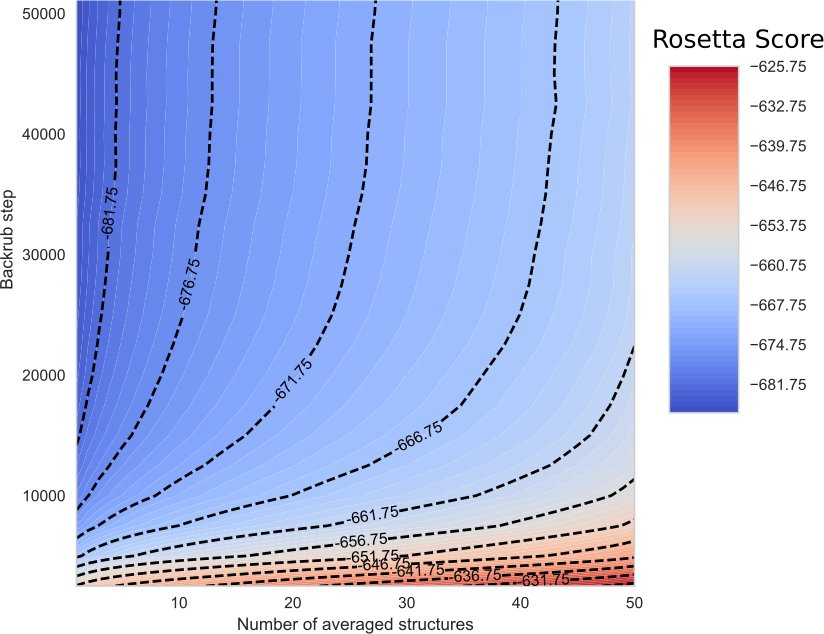
\includegraphics[width=\textwidth,keepaspectratio]{figures/wildtypecomplex-scores-complete.png}
  \caption{
    Contour plot showing the effect of backrub sampling on the average wild-type complex score, for increasing numbers of averaged models. As the number of averaged models is increased along the x-axis, the average total score of the ensemble of wild-type complex models (shown as colored contours in the body of the plot) also increases, as the wild-type complex models are first sorted according to their total scores and included in the averaged ensemble in order of increasing score.
    As the number of backrub sampling steps at which the ensemble is generated increases (along the y-axis), the total score of an ensemble of any number of models tends to decrease, indicating that flex ddG is able to find lower-energy conformations (as measured by the Rosetta energy function) as the simulation progresses. However, using only the lowest energy models does not produce higher correlations with experimental \ddg\ values, as shown in \cref{fig:structs-v-corr-WildTypeComplex-zemu-12-60000-rscript-simplified-t14}.
    Rosetta scores are in Rosetta Energy Units (REU) using the Rosetta Talaris energy function\cite{song_structure-guided_2011,shapovalov_smoothed_2011,omeara_combined_2015}.
  } \label{fig:wildtypecomplex-scores-complete}
\end{figure}

\subimport*{figs-and-tables/}{structs-v-corr-WildTypeComplex-ddg-monomer-16-003-zemu-2}
\subimport*{figs-and-tables/}{structs-v-corr-id-zemu-12-60000-rscript-simplified-t14}

\begin{figure}
  \centering
  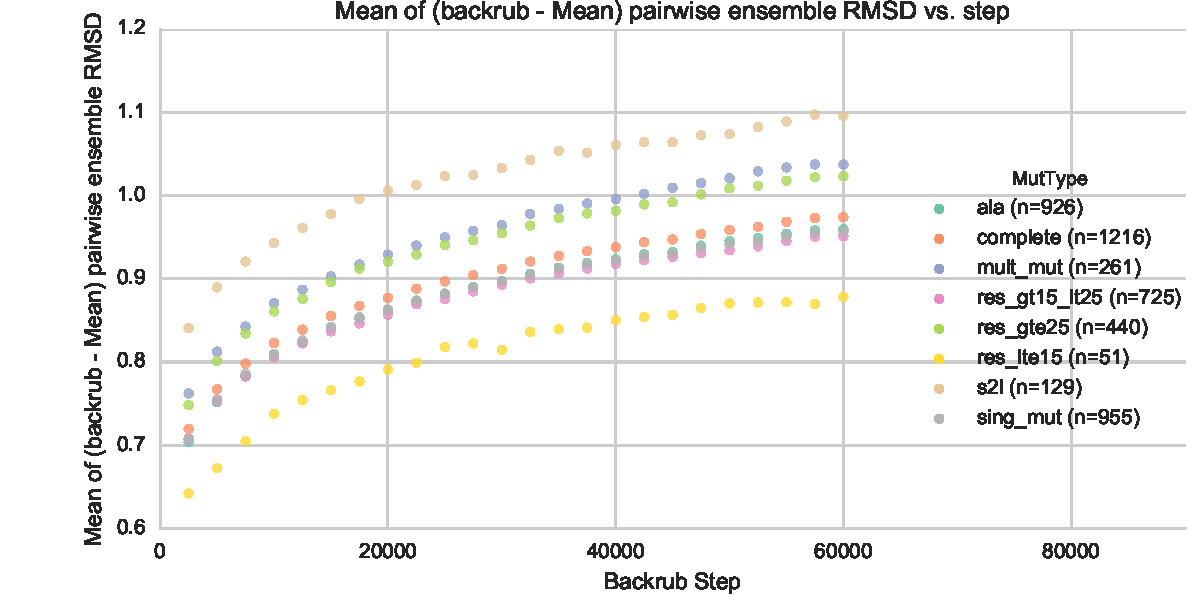
\includegraphics[width=\textwidth,keepaspectratio]{figures/t14-mean-ensemble-error.pdf}
  \caption{
    The average pairwise ensemble RMSD for each ensemble of 50 models is shown versus increasing backrub sampling steps.
    Average pairwise RMSD is computed on all atoms in residues selected as neighborhood pivot residues.
    To calculate pairwise RMSD, this selection of atoms is superimposed onto their positions in the last output model in the backrub trajectory before pairwise RMSDs are computed.
    For all analyzed subsets, including the complete dataset, pairwise ensemble RMSD increases with increasing backrub sampling steps, indicating that the diversity of sampled models (as measured by RMSD) continues to increase past the point around 30k-35k sampling steps where correlation with experimental \ddg\ values levels out. Subset legend: ala = mutation(s) to alanine; complete = complete ZEMu dataset; mult\_mut = multiple mutations (per data point); res\_gt15\_lt25 = resolution of the input wild-type structure $> 1.5\ \AA$ and $< 2.5\ \AA$; res\_gte25 = resolution of the input wild-type structure $>=\ 2.5\ \AA$; res\_lte15 = resolution of the input wild-type structure $<=\ 1.5\ \AA$; s2l = small-to-large mutation(s); sing\_mut = single mutations. N = number of cases in each subset.
  } \label{fig:t14-mean-ensemble} % TODO y axis: mean of pairwise ensemble RMSDs, and remove everything other than complete
\end{figure}

%% HERE

\begin{figure}
  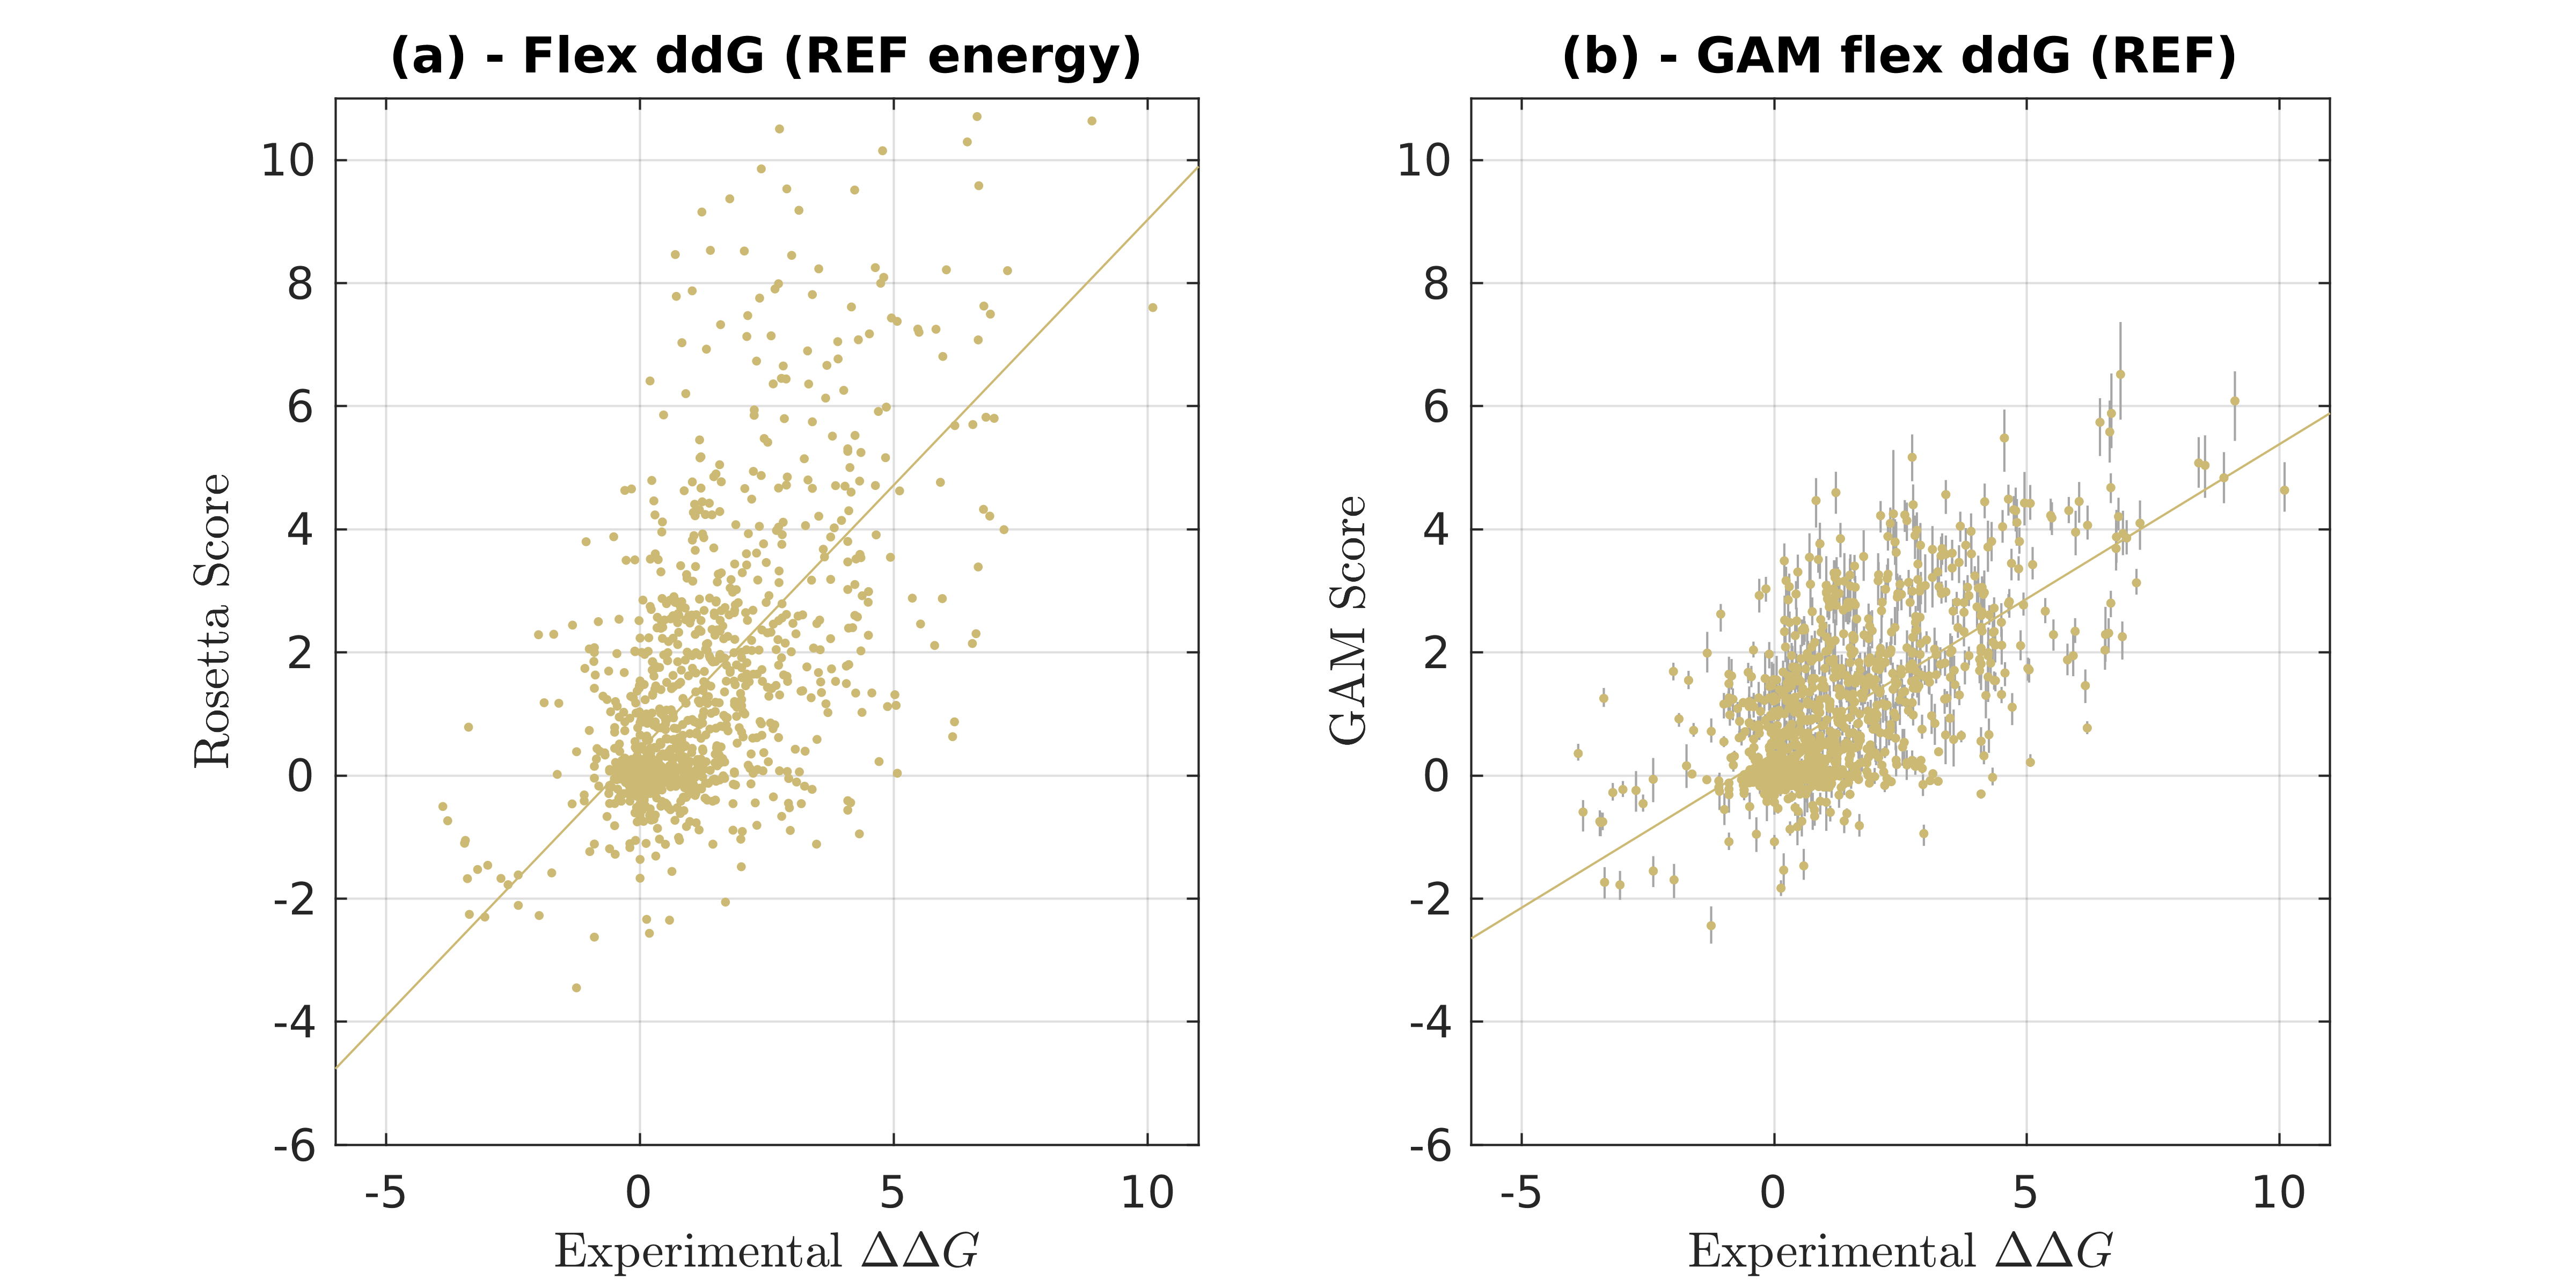
\includegraphics[width=\textwidth,keepaspectratio]{figures/zemu-sigmoid2-corrs-supp.png}
  \caption[]{
    Experimentally determined $\Delta\Delta G$ values (x-axis) versus predictions.
    The error bars in gray represent the range from minimum to maximum fit predicted \ddg\ value for the 1000 sampled GAM (Generalized Additive Model) models.
    A line of best fit is shown.
    \textbf{(a)}: standard Rosetta output (non-fitted REF predictions) vs. experimental \ddg\ values.
    \textbf{(b)}: GAM flex ddG predictions vs. experimental data.
    This plot is analogous to \cref{fig:t14-fit-scatter-main}b in the main text, except that GAM scores are refit from values in Rosetta Energy Units (REU) using the Rosetta REF\cite{alford_rosetta_2017} energy function (instead of Talaris\cite{song_structure-guided_2011,shapovalov_smoothed_2011,omeara_combined_2015}).
  } \label{fig:t14-fit-scatter-supp}
\end{figure}

\begin{figure}
  \centering
  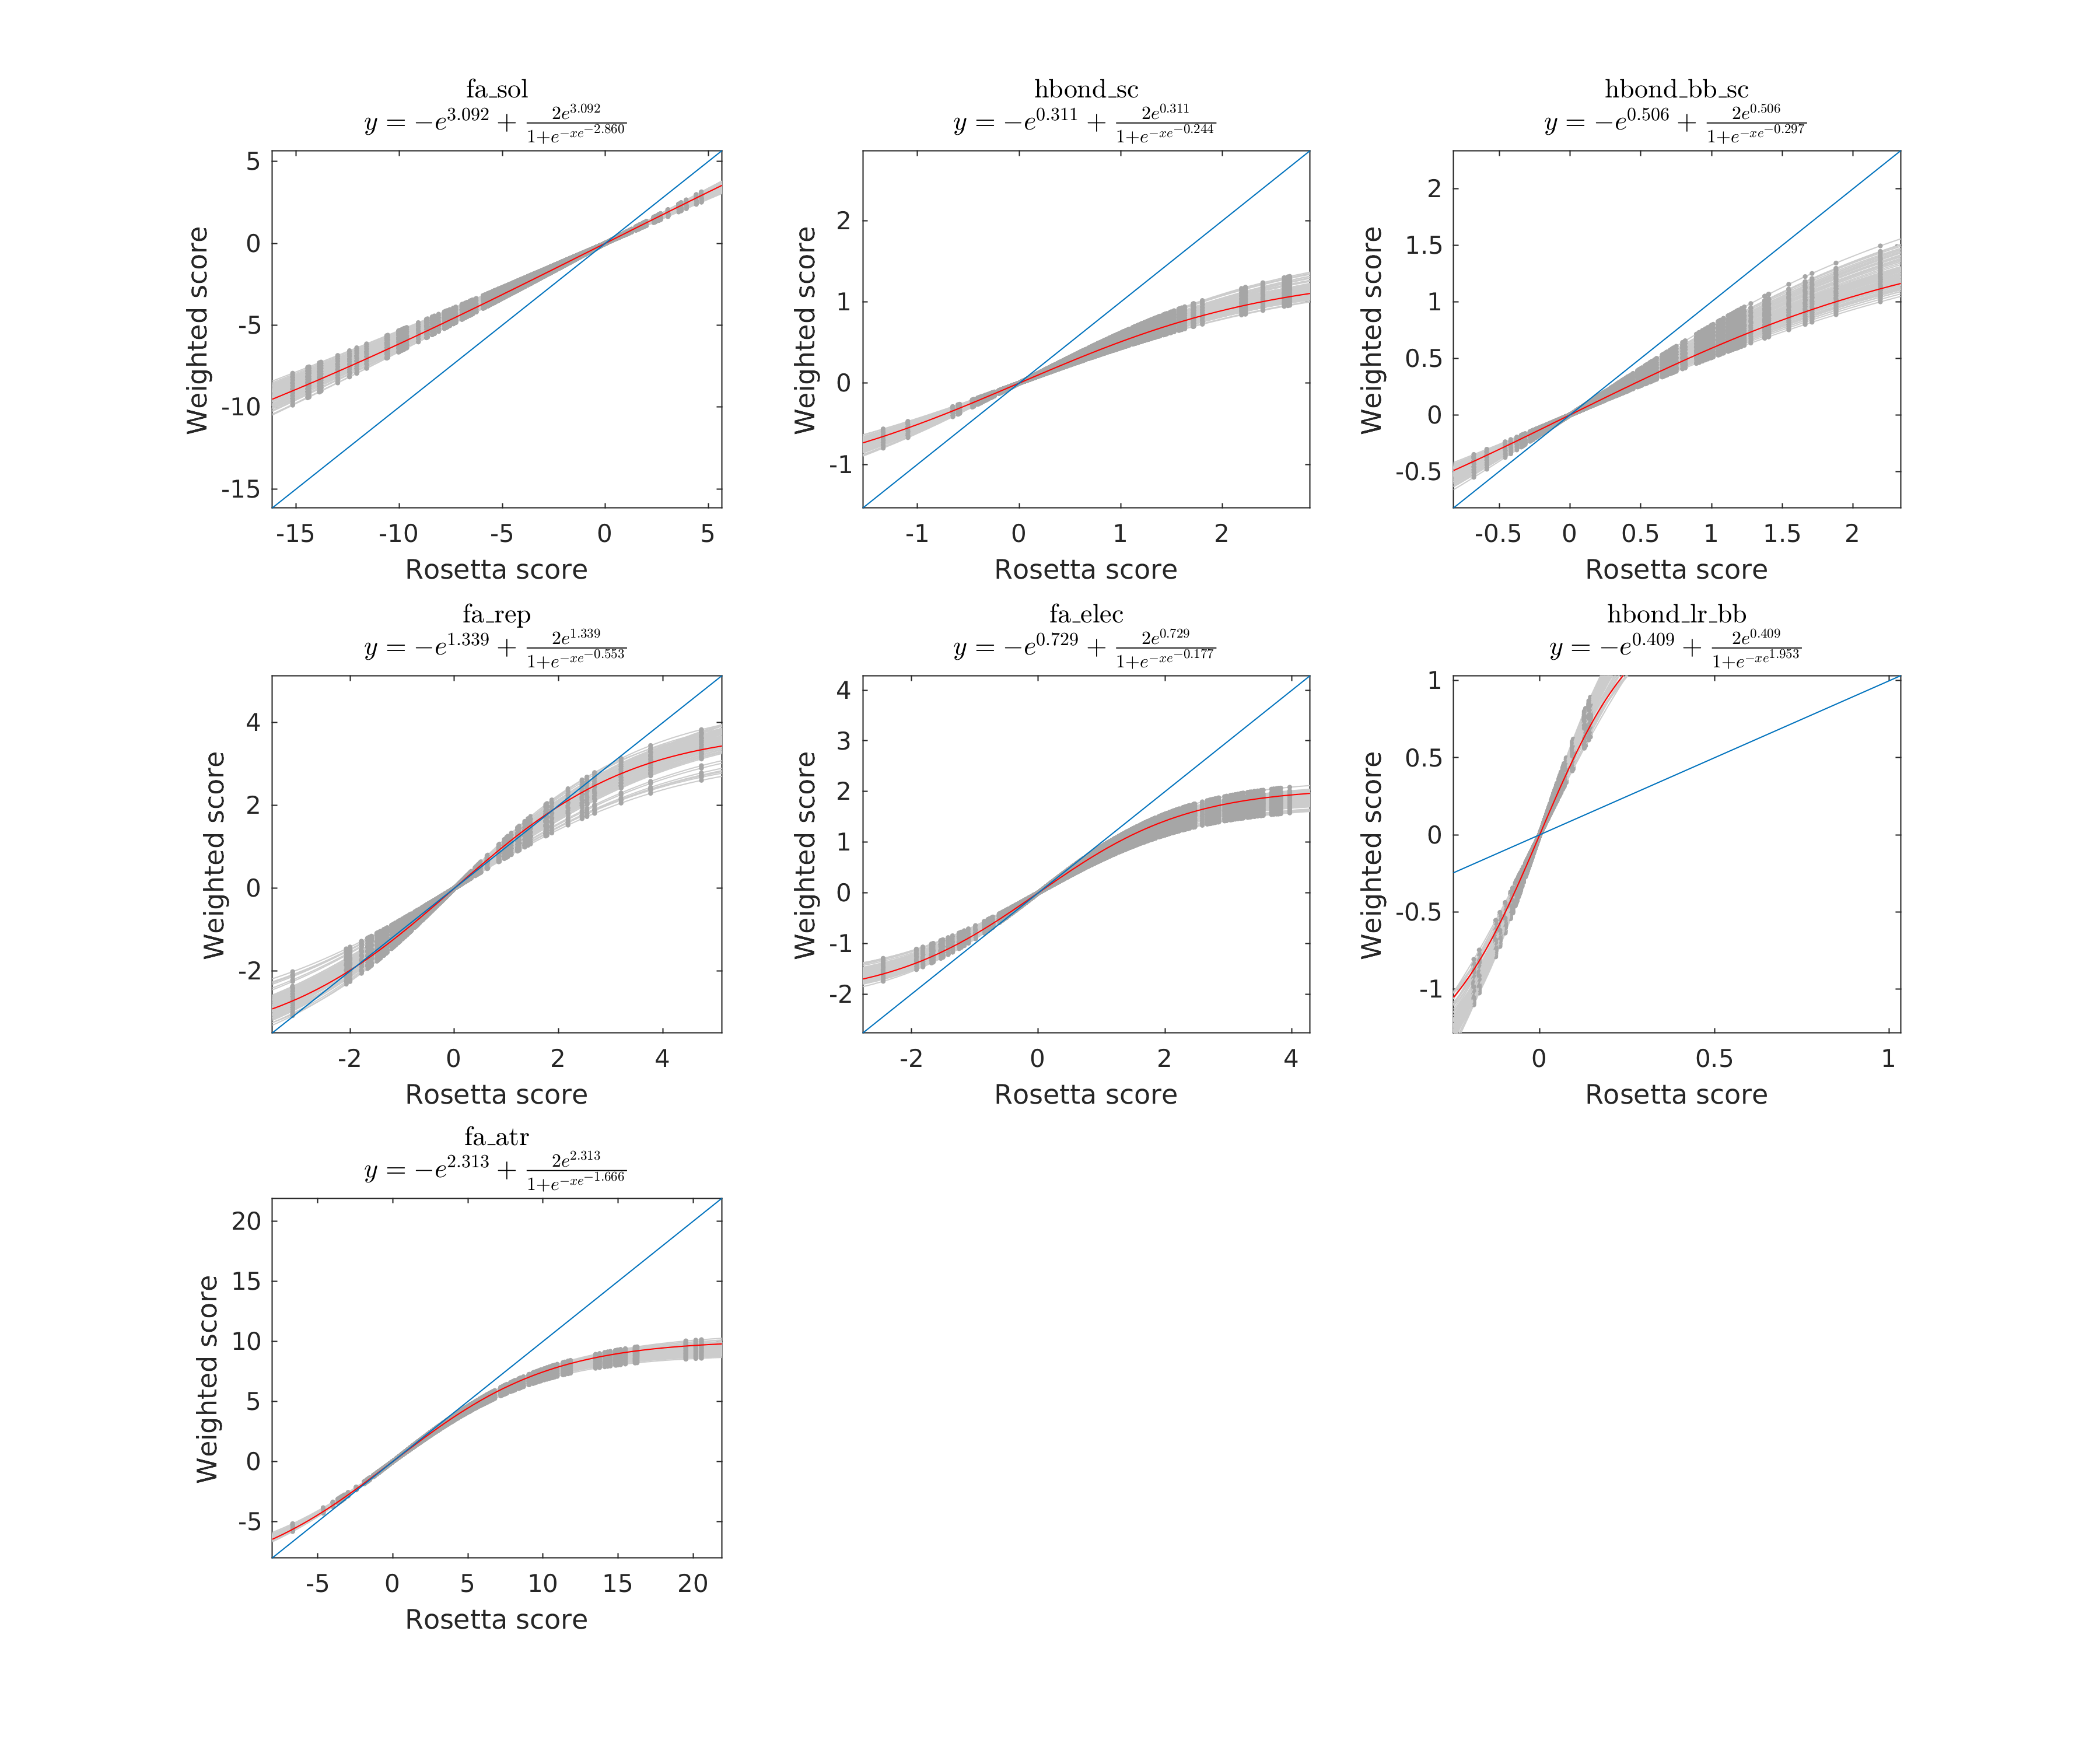
\includegraphics[width=\textwidth,keepaspectratio]{figures/zemu-sigmoid2-tal-feats.png}
  \caption[Sigmoid fit Rosetta score function terms]{
    Sigmoid functions resulting from application of unbiased logistic scaling to individual Rosetta score terms (generated using the flex ddG protocol and the Talaris energy function\cite{song_structure-guided_2011,shapovalov_smoothed_2011,omeara_combined_2015}) in a generalized additive model. Extreme values for most score terms are downweighted, except for long-range hydrogen bond interactions between backbone atoms, which only make minor contributions (hbond\_lr\_bb). % TODO add equation parameters as new table
  } \label{fig:t14-fits-feats}
\end{figure}

\begin{figure}
  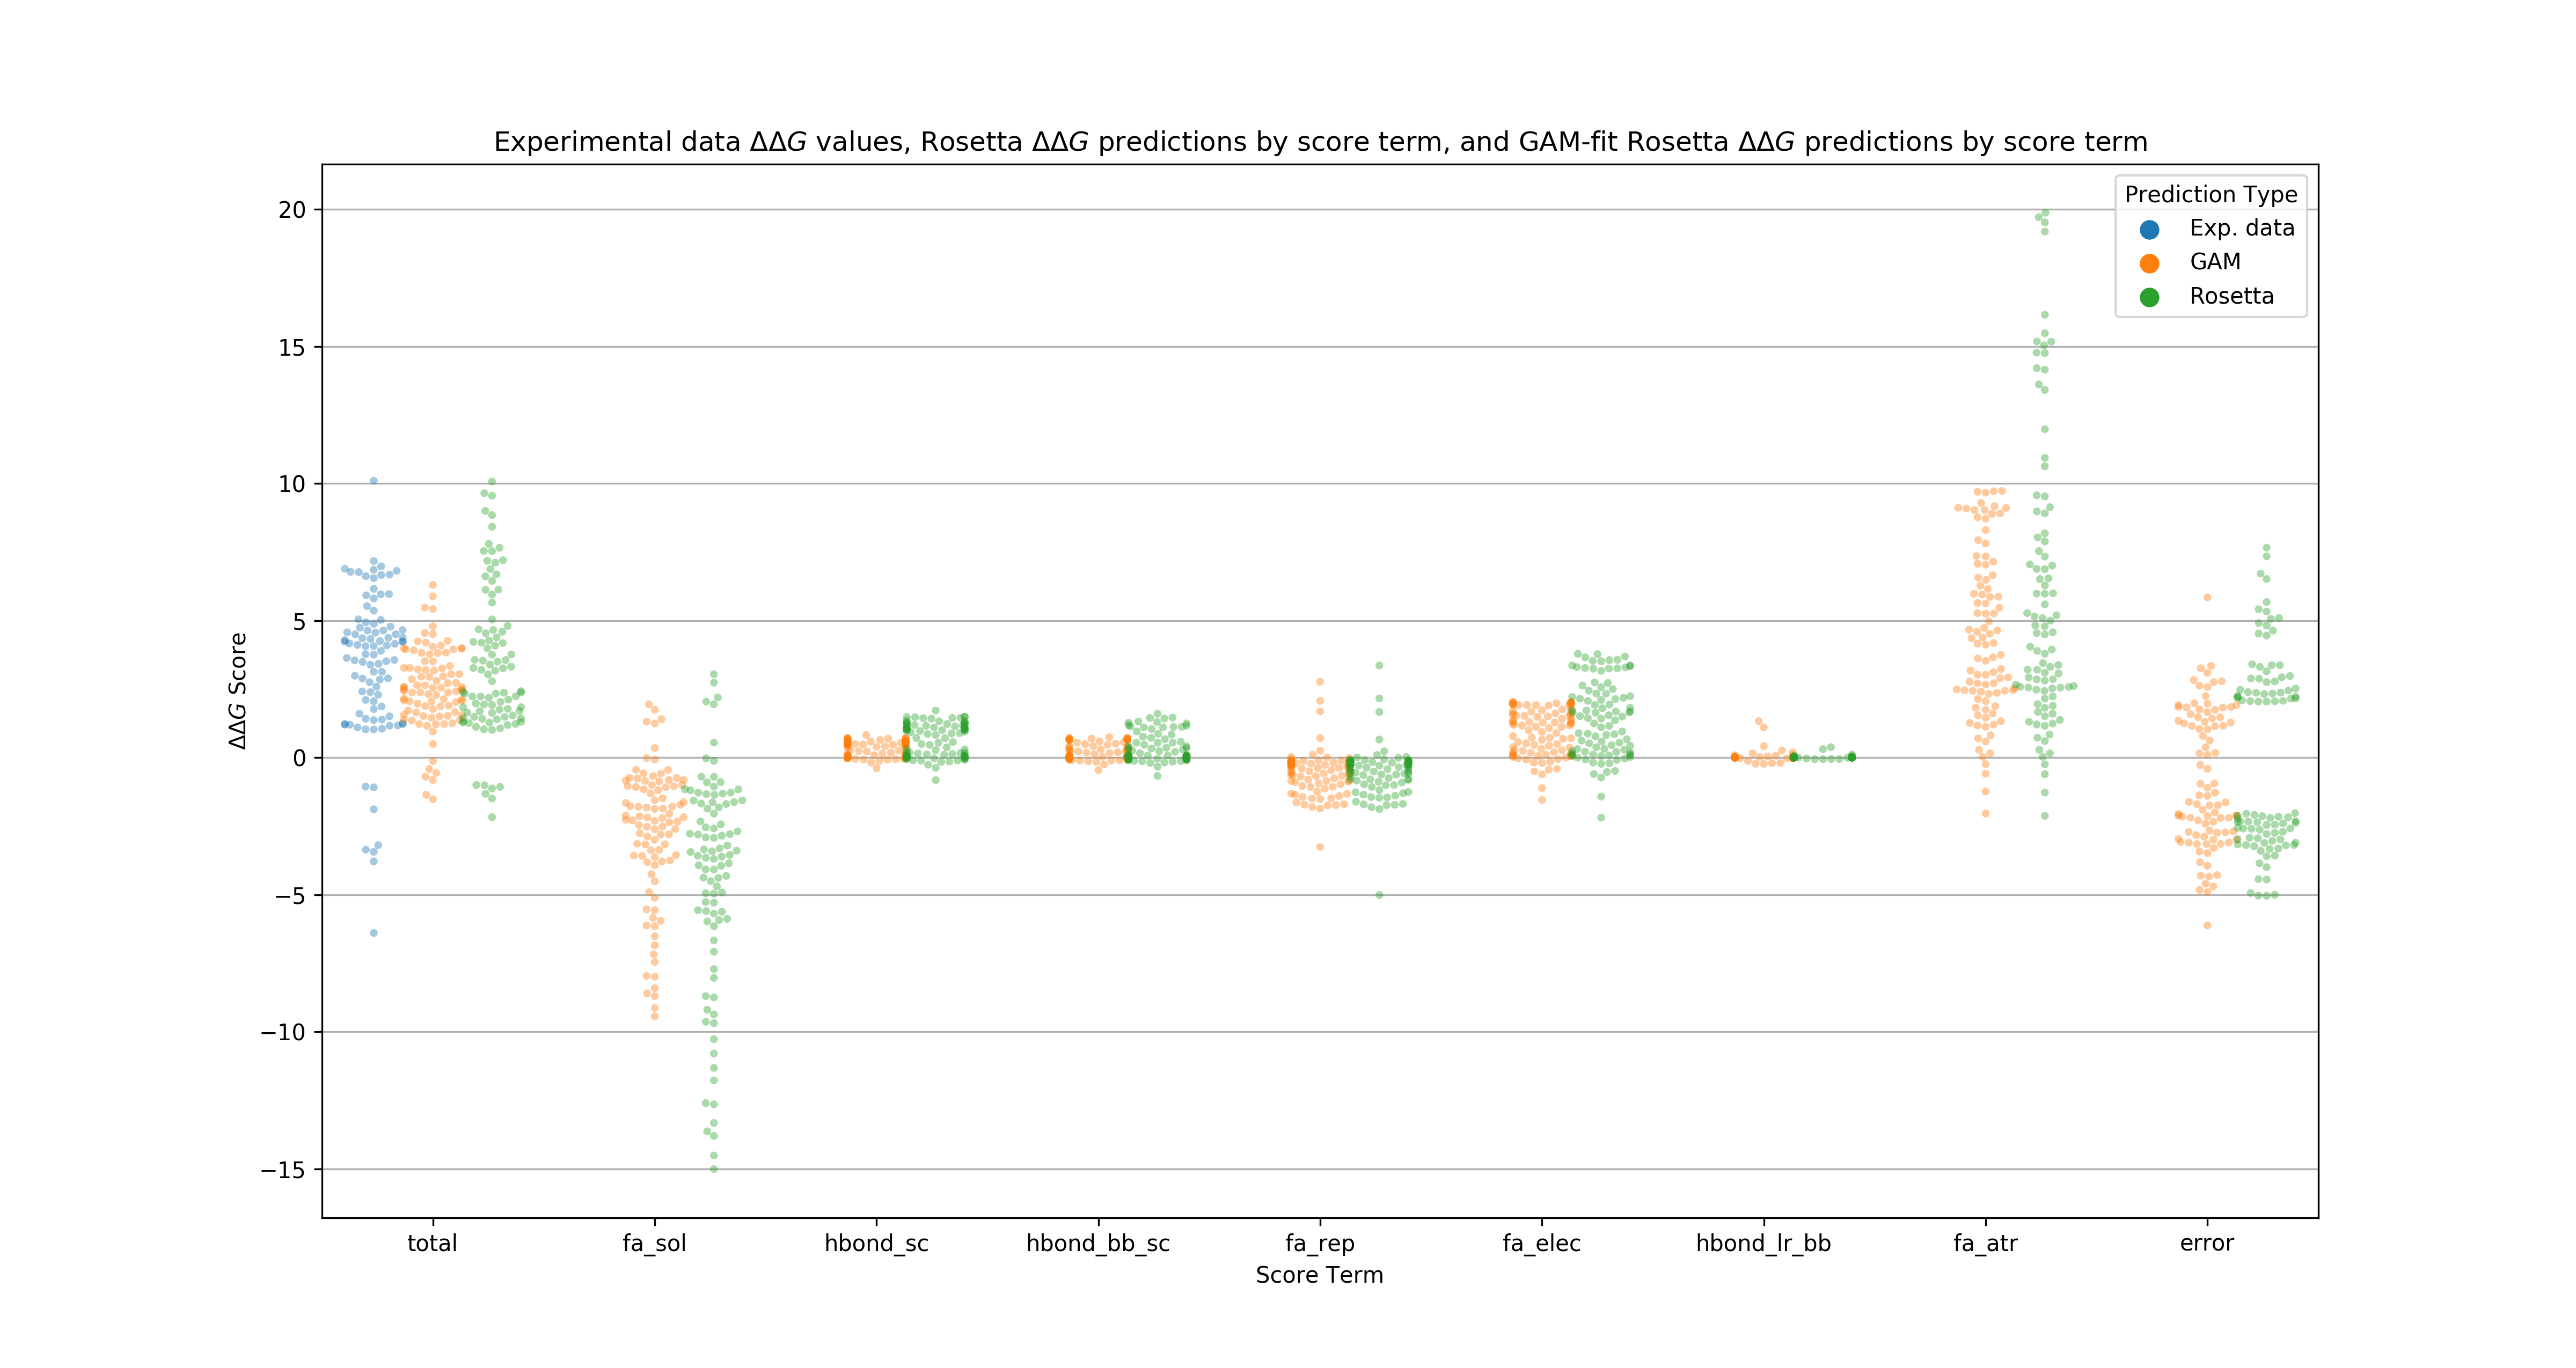
\includegraphics[width=\textwidth,keepaspectratio]{figures/tal-GAM-terms-mpl.png}
  \caption[]{
    Total \ddg\ predictions and partial Rosetta score terms (Talaris energy function\cite{song_structure-guided_2011,shapovalov_smoothed_2011,omeara_combined_2015}). On the far left, total scores for the original Rosetta predictions are shown in green alongside GAM-fit predictions in orange and the experimentally determined values in blue. On the far right, the error ($\Delta\Delta G_{predicted} - \Delta\Delta G_{experimental}$) is shown. Intermediate strips show the 7 partial Rosetta score terms (fa\_sol, hbond\_sc, hbond\_bb\_sc, hbond\_lr\_bb, fa\_rep, fa\_elec, and fa\_atr) which together equal the total \ddg\ score on the far left.
    Points shown are filtered from the complete prediction set according to the following criteria: neutral mutations are removed (-1.0 $<$ experimental \ddg\ or Rosetta predicted \ddg\ score $<$ 1.0). Also removed are points where the absolute value of the error of the original Rosetta prediction is less than 2.0
  } \label{fig:tal-GAM-terms-mpl}
\end{figure}

\clearpage

\renewcommand\tablename{Dataset}
\setcounter{table}{0}

{ \small
\csvreader[
longtable=|c|c|c|p{8cm}|r|,
table head=\caption{Curated ZEMu dataset with experimental \ddg\ values}\label{dst:zemu-filtered}\\\hline
ID & PDB & Res. & Mutations & \ddg\\\hline
\endhead\hline\endfoot,
% \csvlinetotablerow\\\hline
% \endfirsthead\hline
% \csvlinetotablerow\\\hline
% \endhead\hline
% \endfoot,
]
{figures/table-zemu-filtered.csv}
{1=\DataSetID,2=\PDBFileID,3=\Resolution,4=\Mutations,5=\ExperimentalDDG}
{\DataSetID & \PDBFileID & \Resolution & \Mutations & \ExperimentalDDG}
}

\clearpage

\captionof{listing}{
  Flex ddg Rosetta Script implementation
  \label{lst:ddg-script}
}
\inputminted[
linenos=true,
% frame=single,
breaklines
]
{xml}
{listings/ddG-backrub.xml}

\clearpage

\bibliography{references}

\end{document}
\end{suppinfo}

%%%%%%%%%%%%%%%%%%%%%%%%%%%%%%%%%%%%%%%%%%%%%%%%%%%%%%%%%%%%%%%%%%%%%
%% The appropriate \bibliography command should be placed here.
%% Notice that the class file automatically sets \bibliographystyle
%% and also names the section correctly.
%%%%%%%%%%%%%%%%%%%%%%%%%%%%%%%%%%%%%%%%%%%%%%%%%%%%%%%%%%%%%%%%%%%%%
\bibliography{references}

\end{document}
